\documentclass[10pt]{article} % For LaTeX2e
\usepackage{tmlr}
% NOTE: no [accepted] or [preprint] option -- this is a double-blind submission.
% If accepted, instead use the following line for the camera-ready submission:
%\usepackage[accepted]{tmlr}
% To de-anonymize and remove mentions to TMLR (for example for posting to preprint servers), instead use the following:
%\usepackage[preprint]{tmlr}

% Optional math commands from https://github.com/goodfeli/dlbook_notation.
%%%%% NEW MATH DEFINITIONS %%%%%

\usepackage{amsmath,amsfonts,bm}

% Mark sections of captions for referring to divisions of figures
\newcommand{\figleft}{{\em (Left)}}
\newcommand{\figcenter}{{\em (Center)}}
\newcommand{\figright}{{\em (Right)}}
\newcommand{\figtop}{{\em (Top)}}
\newcommand{\figbottom}{{\em (Bottom)}}
\newcommand{\captiona}{{\em (a)}}
\newcommand{\captionb}{{\em (b)}}
\newcommand{\captionc}{{\em (c)}}
\newcommand{\captiond}{{\em (d)}}

% Highlight a newly defined term
\newcommand{\newterm}[1]{{\bf #1}}


% Figure reference, lower-case.
\def\figref#1{figure~\ref{#1}}
% Figure reference, capital. For start of sentence
\def\Figref#1{Figure~\ref{#1}}
\def\twofigref#1#2{figures \ref{#1} and \ref{#2}}
\def\quadfigref#1#2#3#4{figures \ref{#1}, \ref{#2}, \ref{#3} and \ref{#4}}
% Section reference, lower-case.
\def\secref#1{section~\ref{#1}}
% Section reference, capital.
\def\Secref#1{Section~\ref{#1}}
% Reference to two sections.
\def\twosecrefs#1#2{sections \ref{#1} and \ref{#2}}
% Reference to three sections.
\def\secrefs#1#2#3{sections \ref{#1}, \ref{#2} and \ref{#3}}
% Reference to an equation, lower-case.
\def\eqref#1{equation~\ref{#1}}
% Reference to an equation, upper case
\def\Eqref#1{Equation~\ref{#1}}
% A raw reference to an equation---avoid using if possible
\def\plaineqref#1{\ref{#1}}
% Reference to a chapter, lower-case.
\def\chapref#1{chapter~\ref{#1}}
% Reference to an equation, upper case.
\def\Chapref#1{Chapter~\ref{#1}}
% Reference to a range of chapters
\def\rangechapref#1#2{chapters\ref{#1}--\ref{#2}}
% Reference to an algorithm, lower-case.
\def\algref#1{algorithm~\ref{#1}}
% Reference to an algorithm, upper case.
\def\Algref#1{Algorithm~\ref{#1}}
\def\twoalgref#1#2{algorithms \ref{#1} and \ref{#2}}
\def\Twoalgref#1#2{Algorithms \ref{#1} and \ref{#2}}
% Reference to a part, lower case
\def\partref#1{part~\ref{#1}}
% Reference to a part, upper case
\def\Partref#1{Part~\ref{#1}}
\def\twopartref#1#2{parts \ref{#1} and \ref{#2}}

\def\ceil#1{\lceil #1 \rceil}
\def\floor#1{\lfloor #1 \rfloor}
\def\1{\bm{1}}
\newcommand{\train}{\mathcal{D}}
\newcommand{\valid}{\mathcal{D_{\mathrm{valid}}}}
\newcommand{\test}{\mathcal{D_{\mathrm{test}}}}

\def\eps{{\epsilon}}


% Random variables
\def\reta{{\textnormal{$\eta$}}}
\def\ra{{\textnormal{a}}}
\def\rb{{\textnormal{b}}}
\def\rc{{\textnormal{c}}}
\def\rd{{\textnormal{d}}}
\def\re{{\textnormal{e}}}
\def\rf{{\textnormal{f}}}
\def\rg{{\textnormal{g}}}
\def\rh{{\textnormal{h}}}
\def\ri{{\textnormal{i}}}
\def\rj{{\textnormal{j}}}
\def\rk{{\textnormal{k}}}
\def\rl{{\textnormal{l}}}
% rm is already a command, just don't name any random variables m
\def\rn{{\textnormal{n}}}
\def\ro{{\textnormal{o}}}
\def\rp{{\textnormal{p}}}
\def\rq{{\textnormal{q}}}
\def\rr{{\textnormal{r}}}
\def\rs{{\textnormal{s}}}
\def\rt{{\textnormal{t}}}
\def\ru{{\textnormal{u}}}
\def\rv{{\textnormal{v}}}
\def\rw{{\textnormal{w}}}
\def\rx{{\textnormal{x}}}
\def\ry{{\textnormal{y}}}
\def\rz{{\textnormal{z}}}

% Random vectors
\def\rvepsilon{{\mathbf{\epsilon}}}
\def\rvtheta{{\mathbf{\theta}}}
\def\rva{{\mathbf{a}}}
\def\rvb{{\mathbf{b}}}
\def\rvc{{\mathbf{c}}}
\def\rvd{{\mathbf{d}}}
\def\rve{{\mathbf{e}}}
\def\rvf{{\mathbf{f}}}
\def\rvg{{\mathbf{g}}}
\def\rvh{{\mathbf{h}}}
\def\rvu{{\mathbf{i}}}
\def\rvj{{\mathbf{j}}}
\def\rvk{{\mathbf{k}}}
\def\rvl{{\mathbf{l}}}
\def\rvm{{\mathbf{m}}}
\def\rvn{{\mathbf{n}}}
\def\rvo{{\mathbf{o}}}
\def\rvp{{\mathbf{p}}}
\def\rvq{{\mathbf{q}}}
\def\rvr{{\mathbf{r}}}
\def\rvs{{\mathbf{s}}}
\def\rvt{{\mathbf{t}}}
\def\rvu{{\mathbf{u}}}
\def\rvv{{\mathbf{v}}}
\def\rvw{{\mathbf{w}}}
\def\rvx{{\mathbf{x}}}
\def\rvy{{\mathbf{y}}}
\def\rvz{{\mathbf{z}}}

% Elements of random vectors
\def\erva{{\textnormal{a}}}
\def\ervb{{\textnormal{b}}}
\def\ervc{{\textnormal{c}}}
\def\ervd{{\textnormal{d}}}
\def\erve{{\textnormal{e}}}
\def\ervf{{\textnormal{f}}}
\def\ervg{{\textnormal{g}}}
\def\ervh{{\textnormal{h}}}
\def\ervi{{\textnormal{i}}}
\def\ervj{{\textnormal{j}}}
\def\ervk{{\textnormal{k}}}
\def\ervl{{\textnormal{l}}}
\def\ervm{{\textnormal{m}}}
\def\ervn{{\textnormal{n}}}
\def\ervo{{\textnormal{o}}}
\def\ervp{{\textnormal{p}}}
\def\ervq{{\textnormal{q}}}
\def\ervr{{\textnormal{r}}}
\def\ervs{{\textnormal{s}}}
\def\ervt{{\textnormal{t}}}
\def\ervu{{\textnormal{u}}}
\def\ervv{{\textnormal{v}}}
\def\ervw{{\textnormal{w}}}
\def\ervx{{\textnormal{x}}}
\def\ervy{{\textnormal{y}}}
\def\ervz{{\textnormal{z}}}

% Random matrices
\def\rmA{{\mathbf{A}}}
\def\rmB{{\mathbf{B}}}
\def\rmC{{\mathbf{C}}}
\def\rmD{{\mathbf{D}}}
\def\rmE{{\mathbf{E}}}
\def\rmF{{\mathbf{F}}}
\def\rmG{{\mathbf{G}}}
\def\rmH{{\mathbf{H}}}
\def\rmI{{\mathbf{I}}}
\def\rmJ{{\mathbf{J}}}
\def\rmK{{\mathbf{K}}}
\def\rmL{{\mathbf{L}}}
\def\rmM{{\mathbf{M}}}
\def\rmN{{\mathbf{N}}}
\def\rmO{{\mathbf{O}}}
\def\rmP{{\mathbf{P}}}
\def\rmQ{{\mathbf{Q}}}
\def\rmR{{\mathbf{R}}}
\def\rmS{{\mathbf{S}}}
\def\rmT{{\mathbf{T}}}
\def\rmU{{\mathbf{U}}}
\def\rmV{{\mathbf{V}}}
\def\rmW{{\mathbf{W}}}
\def\rmX{{\mathbf{X}}}
\def\rmY{{\mathbf{Y}}}
\def\rmZ{{\mathbf{Z}}}

% Elements of random matrices
\def\ermA{{\textnormal{A}}}
\def\ermB{{\textnormal{B}}}
\def\ermC{{\textnormal{C}}}
\def\ermD{{\textnormal{D}}}
\def\ermE{{\textnormal{E}}}
\def\ermF{{\textnormal{F}}}
\def\ermG{{\textnormal{G}}}
\def\ermH{{\textnormal{H}}}
\def\ermI{{\textnormal{I}}}
\def\ermJ{{\textnormal{J}}}
\def\ermK{{\textnormal{K}}}
\def\ermL{{\textnormal{L}}}
\def\ermM{{\textnormal{M}}}
\def\ermN{{\textnormal{N}}}
\def\ermO{{\textnormal{O}}}
\def\ermP{{\textnormal{P}}}
\def\ermQ{{\textnormal{Q}}}
\def\ermR{{\textnormal{R}}}
\def\ermS{{\textnormal{S}}}
\def\ermT{{\textnormal{T}}}
\def\ermU{{\textnormal{U}}}
\def\ermV{{\textnormal{V}}}
\def\ermW{{\textnormal{W}}}
\def\ermX{{\textnormal{X}}}
\def\ermY{{\textnormal{Y}}}
\def\ermZ{{\textnormal{Z}}}

% Vectors
\def\vzero{{\bm{0}}}
\def\vone{{\bm{1}}}
\def\vmu{{\bm{\mu}}}
\def\vtheta{{\bm{\theta}}}
\def\va{{\bm{a}}}
\def\vb{{\bm{b}}}
\def\vc{{\bm{c}}}
\def\vd{{\bm{d}}}
\def\ve{{\bm{e}}}
\def\vf{{\bm{f}}}
\def\vg{{\bm{g}}}
\def\vh{{\bm{h}}}
\def\vi{{\bm{i}}}
\def\vj{{\bm{j}}}
\def\vk{{\bm{k}}}
\def\vl{{\bm{l}}}
\def\vm{{\bm{m}}}
\def\vn{{\bm{n}}}
\def\vo{{\bm{o}}}
\def\vp{{\bm{p}}}
\def\vq{{\bm{q}}}
\def\vr{{\bm{r}}}
\def\vs{{\bm{s}}}
\def\vt{{\bm{t}}}
\def\vu{{\bm{u}}}
\def\vv{{\bm{v}}}
\def\vw{{\bm{w}}}
\def\vx{{\bm{x}}}
\def\vy{{\bm{y}}}
\def\vz{{\bm{z}}}

% Elements of vectors
\def\evalpha{{\alpha}}
\def\evbeta{{\beta}}
\def\evepsilon{{\epsilon}}
\def\evlambda{{\lambda}}
\def\evomega{{\omega}}
\def\evmu{{\mu}}
\def\evpsi{{\psi}}
\def\evsigma{{\sigma}}
\def\evtheta{{\theta}}
\def\eva{{a}}
\def\evb{{b}}
\def\evc{{c}}
\def\evd{{d}}
\def\eve{{e}}
\def\evf{{f}}
\def\evg{{g}}
\def\evh{{h}}
\def\evi{{i}}
\def\evj{{j}}
\def\evk{{k}}
\def\evl{{l}}
\def\evm{{m}}
\def\evn{{n}}
\def\evo{{o}}
\def\evp{{p}}
\def\evq{{q}}
\def\evr{{r}}
\def\evs{{s}}
\def\evt{{t}}
\def\evu{{u}}
\def\evv{{v}}
\def\evw{{w}}
\def\evx{{x}}
\def\evy{{y}}
\def\evz{{z}}

% Matrix
\def\mA{{\bm{A}}}
\def\mB{{\bm{B}}}
\def\mC{{\bm{C}}}
\def\mD{{\bm{D}}}
\def\mE{{\bm{E}}}
\def\mF{{\bm{F}}}
\def\mG{{\bm{G}}}
\def\mH{{\bm{H}}}
\def\mI{{\bm{I}}}
\def\mJ{{\bm{J}}}
\def\mK{{\bm{K}}}
\def\mL{{\bm{L}}}
\def\mM{{\bm{M}}}
\def\mN{{\bm{N}}}
\def\mO{{\bm{O}}}
\def\mP{{\bm{P}}}
\def\mQ{{\bm{Q}}}
\def\mR{{\bm{R}}}
\def\mS{{\bm{S}}}
\def\mT{{\bm{T}}}
\def\mU{{\bm{U}}}
\def\mV{{\bm{V}}}
\def\mW{{\bm{W}}}
\def\mX{{\bm{X}}}
\def\mY{{\bm{Y}}}
\def\mZ{{\bm{Z}}}
\def\mBeta{{\bm{\beta}}}
\def\mPhi{{\bm{\Phi}}}
\def\mLambda{{\bm{\Lambda}}}
\def\mSigma{{\bm{\Sigma}}}

% Tensor
\DeclareMathAlphabet{\mathsfit}{\encodingdefault}{\sfdefault}{m}{sl}
\SetMathAlphabet{\mathsfit}{bold}{\encodingdefault}{\sfdefault}{bx}{n}
\newcommand{\tens}[1]{\bm{\mathsfit{#1}}}
\def\tA{{\tens{A}}}
\def\tB{{\tens{B}}}
\def\tC{{\tens{C}}}
\def\tD{{\tens{D}}}
\def\tE{{\tens{E}}}
\def\tF{{\tens{F}}}
\def\tG{{\tens{G}}}
\def\tH{{\tens{H}}}
\def\tI{{\tens{I}}}
\def\tJ{{\tens{J}}}
\def\tK{{\tens{K}}}
\def\tL{{\tens{L}}}
\def\tM{{\tens{M}}}
\def\tN{{\tens{N}}}
\def\tO{{\tens{O}}}
\def\tP{{\tens{P}}}
\def\tQ{{\tens{Q}}}
\def\tR{{\tens{R}}}
\def\tS{{\tens{S}}}
\def\tT{{\tens{T}}}
\def\tU{{\tens{U}}}
\def\tV{{\tens{V}}}
\def\tW{{\tens{W}}}
\def\tX{{\tens{X}}}
\def\tY{{\tens{Y}}}
\def\tZ{{\tens{Z}}}


% Graph
\def\gA{{\mathcal{A}}}
\def\gB{{\mathcal{B}}}
\def\gC{{\mathcal{C}}}
\def\gD{{\mathcal{D}}}
\def\gE{{\mathcal{E}}}
\def\gF{{\mathcal{F}}}
\def\gG{{\mathcal{G}}}
\def\gH{{\mathcal{H}}}
\def\gI{{\mathcal{I}}}
\def\gJ{{\mathcal{J}}}
\def\gK{{\mathcal{K}}}
\def\gL{{\mathcal{L}}}
\def\gM{{\mathcal{M}}}
\def\gN{{\mathcal{N}}}
\def\gO{{\mathcal{O}}}
\def\gP{{\mathcal{P}}}
\def\gQ{{\mathcal{Q}}}
\def\gR{{\mathcal{R}}}
\def\gS{{\mathcal{S}}}
\def\gT{{\mathcal{T}}}
\def\gU{{\mathcal{U}}}
\def\gV{{\mathcal{V}}}
\def\gW{{\mathcal{W}}}
\def\gX{{\mathcal{X}}}
\def\gY{{\mathcal{Y}}}
\def\gZ{{\mathcal{Z}}}

% Sets
\def\sA{{\mathbb{A}}}
\def\sB{{\mathbb{B}}}
\def\sC{{\mathbb{C}}}
\def\sD{{\mathbb{D}}}
% Don't use a set called E, because this would be the same as our symbol
% for expectation.
\def\sF{{\mathbb{F}}}
\def\sG{{\mathbb{G}}}
\def\sH{{\mathbb{H}}}
\def\sI{{\mathbb{I}}}
\def\sJ{{\mathbb{J}}}
\def\sK{{\mathbb{K}}}
\def\sL{{\mathbb{L}}}
\def\sM{{\mathbb{M}}}
\def\sN{{\mathbb{N}}}
\def\sO{{\mathbb{O}}}
\def\sP{{\mathbb{P}}}
\def\sQ{{\mathbb{Q}}}
\def\sR{{\mathbb{R}}}
\def\sS{{\mathbb{S}}}
\def\sT{{\mathbb{T}}}
\def\sU{{\mathbb{U}}}
\def\sV{{\mathbb{V}}}
\def\sW{{\mathbb{W}}}
\def\sX{{\mathbb{X}}}
\def\sY{{\mathbb{Y}}}
\def\sZ{{\mathbb{Z}}}

% Entries of a matrix
\def\emLambda{{\Lambda}}
\def\emA{{A}}
\def\emB{{B}}
\def\emC{{C}}
\def\emD{{D}}
\def\emE{{E}}
\def\emF{{F}}
\def\emG{{G}}
\def\emH{{H}}
\def\emI{{I}}
\def\emJ{{J}}
\def\emK{{K}}
\def\emL{{L}}
\def\emM{{M}}
\def\emN{{N}}
\def\emO{{O}}
\def\emP{{P}}
\def\emQ{{Q}}
\def\emR{{R}}
\def\emS{{S}}
\def\emT{{T}}
\def\emU{{U}}
\def\emV{{V}}
\def\emW{{W}}
\def\emX{{X}}
\def\emY{{Y}}
\def\emZ{{Z}}
\def\emSigma{{\Sigma}}

% entries of a tensor
% Same font as tensor, without \bm wrapper
\newcommand{\etens}[1]{\mathsfit{#1}}
\def\etLambda{{\etens{\Lambda}}}
\def\etA{{\etens{A}}}
\def\etB{{\etens{B}}}
\def\etC{{\etens{C}}}
\def\etD{{\etens{D}}}
\def\etE{{\etens{E}}}
\def\etF{{\etens{F}}}
\def\etG{{\etens{G}}}
\def\etH{{\etens{H}}}
\def\etI{{\etens{I}}}
\def\etJ{{\etens{J}}}
\def\etK{{\etens{K}}}
\def\etL{{\etens{L}}}
\def\etM{{\etens{M}}}
\def\etN{{\etens{N}}}
\def\etO{{\etens{O}}}
\def\etP{{\etens{P}}}
\def\etQ{{\etens{Q}}}
\def\etR{{\etens{R}}}
\def\etS{{\etens{S}}}
\def\etT{{\etens{T}}}
\def\etU{{\etens{U}}}
\def\etV{{\etens{V}}}
\def\etW{{\etens{W}}}
\def\etX{{\etens{X}}}
\def\etY{{\etens{Y}}}
\def\etZ{{\etens{Z}}}

% The true underlying data generating distribution
\newcommand{\pdata}{p_{\rm{data}}}
% The empirical distribution defined by the training set
\newcommand{\ptrain}{\hat{p}_{\rm{data}}}
\newcommand{\Ptrain}{\hat{P}_{\rm{data}}}
% The model distribution
\newcommand{\pmodel}{p_{\rm{model}}}
\newcommand{\Pmodel}{P_{\rm{model}}}
\newcommand{\ptildemodel}{\tilde{p}_{\rm{model}}}
% Stochastic autoencoder distributions
\newcommand{\pencode}{p_{\rm{encoder}}}
\newcommand{\pdecode}{p_{\rm{decoder}}}
\newcommand{\precons}{p_{\rm{reconstruct}}}

\newcommand{\laplace}{\mathrm{Laplace}} % Laplace distribution

\newcommand{\E}{\mathbb{E}}
\newcommand{\Ls}{\mathcal{L}}
\newcommand{\R}{\mathbb{R}}
\newcommand{\emp}{\tilde{p}}
\newcommand{\lr}{\alpha}
\newcommand{\reg}{\lambda}
\newcommand{\rect}{\mathrm{rectifier}}
\newcommand{\softmax}{\mathrm{softmax}}
\newcommand{\sigmoid}{\sigma}
\newcommand{\softplus}{\zeta}
\newcommand{\KL}{D_{\mathrm{KL}}}
\newcommand{\Var}{\mathrm{Var}}
\newcommand{\standarderror}{\mathrm{SE}}
\newcommand{\Cov}{\mathrm{Cov}}
% Wolfram Mathworld says $L^2$ is for function spaces and $\ell^2$ is for vectors
% But then they seem to use $L^2$ for vectors throughout the site, and so does
% wikipedia.
\newcommand{\normlzero}{L^0}
\newcommand{\normlone}{L^1}
\newcommand{\normltwo}{L^2}
\newcommand{\normlp}{L^p}
\newcommand{\normmax}{L^\infty}

\newcommand{\parents}{Pa} % See usage in notation.tex. Chosen to match Daphne's book.

\DeclareMathOperator*{\argmax}{arg\,max}
\DeclareMathOperator*{\argmin}{arg\,min}

\DeclareMathOperator{\sign}{sign}
\DeclareMathOperator{\Tr}{Tr}
\let\ab\allowbreak


\usepackage{graphicx}
\usepackage{amssymb}
\usepackage{url}
\usepackage{hyperref}

% ----------------------------------------------------------------------
% Draft provenance (working-draft front matter; kept as a comment so that
% it is not typeset in the submission PDF).
%
% Complete draft v3 -- Sections 1-7 + Reproducibility
% 2026-10-27 (v3: adversarial review applied -- see results/ind48_robust_report.md).
% Numbers are final from results/protocol_a_fig3_report.md,
% results/r1_final_report.md, results/ind_validation_report.md,
% results/bootstrap_ci_report.md, results/multiarch_report.md,
% results/ind48_robust_report.md, and runs/glue_own48_results.json.
% ----------------------------------------------------------------------

\title{When Do Geometric Markers Predict Generalization? A Controlled Analysis of Task-Relevance and Shift Type}

% Authors must not appear in the submitted version. They are hidden
% automatically as long as the tmlr package is used without the [accepted]
% or [preprint] options.
\author{\name Anonymous Authors \AND \addr Anonymous Affiliation}

% Camera-ready only:
%\def\month{MM}  % Insert correct month for camera-ready version
%\def\year{YYYY} % Insert correct year for camera-ready version
%\def\openreview{\url{https://openreview.net/forum?id=XXXX}} % Insert correct link to OpenReview for camera-ready version

% Section cross-reference shorthands used throughout the paper.
% NOTE: \secref and \Secref are already defined by math_commands.tex (as
% "section~\ref{...}"), so we use distinct names here. \srcref renders the
% section sign directly, matching the draft's "§4.7" notation.
\newcommand{\srcref}[1]{\S\ref{#1}}
\newcommand{\limref}[1]{Limitations~\ref{#1}}
\newcommand{\okmark}{\ensuremath{\checkmark}}
\newcommand{\nomark}{\ensuremath{\times}}

\begin{document}

\maketitle

\begin{abstract}
% NOTE: TMLR requires the abstract to be limited to a single paragraph (see the
% official template, main.tex: "The abstract must be limited to one paragraph").
% The source draft wrote the abstract as seven paragraphs; they are merged here
% into one paragraph with no sentence or number removed.
Neural representation geometry has recently been proposed as a cheap, training-free proxy for predicting a model's generalization performance. Recent work \citep{chou2026diagnosing} shows that geometry-derived markers such as the effective dimension ($D_{\mathrm{eff}}$) correlate strongly with out-of-distribution (OOD) accuracy and outperform in-distribution (ID) test accuracy as a model-selection criterion. We argue that such comparisons require three controls that are rarely applied: (i) they must be made within a subset of models with near-identical ID accuracy, since ID accuracy is the very quantity the markers are meant to supplement; (ii) architecture main effects must be removed, since architecture families differ systematically in both ID accuracy and representational geometry; and (iii) marker strength must be reported with rank-based statistics alongside Pearson correlations, since a strong Pearson coefficient alone can be driven by a few extreme points. We formalize these as a four-condition protocol --- ID matching, group residualization, dual correlation statistics, and cross-group sign consistency --- and report what it reveals when applied to the per-model measurements released with the original study (5 architectures, 224 models: each architecture trained on its own $4$ learning rates $\times$ $4$ weight decays $\times$ $2$--$3$ seeds, with the union of hyperparameter values spanning 13 learning rates and 9 weight decays), to a second release of that study (80 models, 6 corruption scenarios), and to 78 models we trained ourselves across three architectures. Three findings emerge. (i) \textbf{The task-relevant markers survive all four controls.} $D_{\mathrm{eff}}$ retains a strong, rank-consistent, sign-consistent association with OOD accuracy under the ID-matched, architecture-adjusted protocol ($r = +0.93$, $\rho = +0.85$, $p < 10^{-4}$, positive in all five architectures), with 100\% bootstrap robustness. This is not a Simpson's paradox. (ii) \textbf{The accuracy baseline is not a stable reference point.} At fixed ID accuracy with architecture effects removed, the sign of the ID-accuracy association is not consistent across populations: on the two releases of the original study it is positive on one ($+0.39$, 95\% CI $[+0.22,+0.62]$) and negative on the other ($-0.63$, 95\% CI $[-0.83,-0.42]$), and on our own 48 models it is negative in aggregate but \emph{flips sign within training families}, failing the protocol's own sign-consistency condition. An accuracy baseline whose sign depends on the population cannot anchor a ``markers beat accuracy'' claim in either direction. (iii) \textbf{The markers' advantage is conditional on the shift type.} Under photometric and structural corruptions (fog, brightness, contrast), ID accuracy is restored as the strongest predictor ($\rho_{\text{resid}} = +0.77$ to $+0.97$, ranked 1st of 12 markers); under noise and compression corruptions it collapses ($\rho_{\text{resid}} = -0.09$ to $+0.22$, ranked 6th--11th) and geometric markers take over. A single aggregate statement about corruption robustness averages over two opposite regimes. A third, independent observation explains why the baseline behaves this way. On our 48 self-trained models, geometric markers and ID accuracy are \textbf{nearly uncorrelated with each other} ($-0.17$ to $-0.04$) while the markers correlate at $+0.90$ to $+0.95$ with OOD accuracy and ID accuracy does not ($-0.05$). The two candidate signals measure different things --- how well the network fits the training distribution versus how its learned representation is organised --- and on class-level shifts only the second is informative. We conclude that the predictive value of representational-geometry markers is conditional on both the task-relevance of the marker and the type of distribution shift, and that claims that geometric markers ``replace'' ID accuracy must state these qualifications explicitly. We release the control protocol as a reusable diagnostic and validate it on independently trained model families across two class-level shifts, where the baseline's sign instability replicates.
\end{abstract}

\section{Introduction}
\label{sec:intro}

Predicting how a trained network will behave beyond its training distribution is a long-standing problem with growing practical stakes. Test accuracy on held-out in-distribution (ID) data is the default summary of model quality, but it is exactly the quantity that fails to anticipate out-of-distribution (OOD) behavior. A promising alternative has emerged from the study of representational geometry: rather than evaluating a model on data, one measures geometric properties of its internal representations --- class manifolds, their dimensionality, radius, and alignment --- and asks whether these quantities track (or even forecast) downstream performance.

Two families of geometric markers have been explored. The first uses task-agnostic statistics of the feature distribution: participation ratio, mean pairwise distances and angles, covariance sparsity. The second uses task-relevant quantities derived from manifold capacity theory: the GLUE framework \citep{chou2025feature} defines, for each class manifold, an effective dimension $D_{\mathrm{eff}}$, effective radius $R_{\mathrm{eff}}$, and effective utility $\Psi_{\mathrm{eff}}$, computed from anchor points of a quadratic program that mirrors linear separability. Recent work by \citet{chou2026diagnosing} --- hereafter ``the original study'' --- reports that these task-relevant markers, measured on ID data, forecast OOD generalization failures, and do so more reliably than ID test accuracy itself.

The comparison at the heart of that claim --- geometric markers versus ID accuracy --- is the subject of this paper. We show that as stated, the comparison is not yet well defined, and that once it is made well defined, both parts of the claim change: the markers' advantage grows, but so does the set of conditions under which it fails.

\textbf{Three unhandled confounds.} Comparisons of a proposed proxy against an accuracy baseline are typically made on a pooled correlation over a heterogeneous model population: five architectures, each trained under multiple hyperparameter settings. This design leaves three confounds untreated. First, ID accuracy is not controlled: if two architecture families differ systematically in both ID accuracy and OOD transfer, the pooled correlation between ID accuracy and OOD performance is dominated by between-architecture differences, not by the within-architecture relationship that model selection actually relies on. Second, no per-group sign consistency is checked: a pooled coefficient can be positive while every within-architecture coefficient is negative --- the textbook setting of Simpson's paradox. Third, shift type is not treated as a variable: ``OOD'' spans class-level shifts (new object categories) and corruption shifts (photometric and structural degradations), and there is no a priori reason the same marker should dominate under both.

\textbf{What we find.} We re-analyze the per-model measurements released with the original study --- 224 models across five architectures, each architecture trained on its own $4\times4$ learning-rate/weight-decay grid with 2--3 seeds (the union of hyperparameter values spans 13 learning rates and 9 weight decays; this is a union of per-architecture grids, not a Cartesian product), including the study's own released values of $D_{\mathrm{eff}}$, $R_{\mathrm{eff}}$, and $\Psi_{\mathrm{eff}}$ --- under a protocol that (a) restricts attention to models with near-identical ID accuracy ($\pm1$ percentage point), (b) residualizes out architecture main effects, (c) reports Pearson and Spearman coefficients jointly and requires them to agree, and (d) requires the sign of each association to be consistent across architectures. We then apply the identical protocol to the study's second release (80 models, 6 corruption scenarios) and to 78 models we trained ourselves across three architectures and two class-level shifts. Three findings emerge.

1. \emph{The geometric markers survive the controls.} Within the ID-matched, architecture-adjusted subset ($n=106$), $D_{\mathrm{eff}}$ remains strongly associated with OOD accuracy ($r=+0.93$, $\rho=+0.85$, both $p<10^{-4}$), with consistent sign in all five architectures and 100\% bootstrap robustness. The effect is real, not an aggregation artifact.

2. \emph{The baseline is worse than weak --- it is not a stable reference point.} On the 224-model release, ID accuracy has essentially no pooled association with OOD accuracy ($r=-0.05$); after architecture adjustment its Pearson coefficient is $+0.39$. On the study's second release (80 models, 6 corruption scenarios), the same protocol yields $r=-0.63$. Stratified bootstrap over the full pipeline gives 95\% confidence intervals $[+0.22, +0.62]$ and $[-0.83, -0.42]$ on the two datasets respectively: both exclude zero, in opposite directions. On our own 48 models the aggregate is negative ($-0.44$) but the sign \emph{flips within training families}, so the baseline fails the protocol's own sign-consistency condition there. More fundamentally, on those same 48 models the baseline is \emph{nearly uncorrelated with the geometric markers} ($-0.05$ with OOD accuracy, $-0.17$ with marker values), so the two candidate signals are not competing measurements of a common quantity --- they are largely independent, and only one of them tracks class-level transfer. An ID-accuracy baseline whose sign depends on the population cannot anchor a ``markers beat the baseline'' claim in either direction.

3. \emph{The markers' advantage is shift-type dependent.} Under photometric and structural corruptions (fog, brightness, contrast), ID accuracy is again the strongest predictor of corruption accuracy ($\rho_{\text{resid}}$ up to $+0.97$, 1st of 12); under noise and compression corruptions it fails ($\rho_{\text{resid}}$ between $-0.09$ and $+0.22$, ranked 6th--11th), and geometry-derived markers take over. The original study reports the corruption case as a single aggregate; splitting it reveals that both halves of the aggregate statement hold for disjoint reasons. We report this decomposition under both an uncontrolled and a fully controlled instrument, and the split survives either way.

\textbf{Independent validation.} Because all of the above analyzes the original authors' own released measurements, we additionally train 48 ResNet-18 models under a $4\times4$ learning-rate/weight-decay grid with 3 seeds, plus 16 models each of ShuffleNetV2-x1.0 \citep{ma2018shufflenet} and RegNetY-400MF \citep{radosavovic2020designing}, and run the identical protocol with publicly computable markers on two independent class-level shifts: CIFAR-100 and Tiny-ImageNet \citep{le2015tiny} linear probes. The baseline's negative aggregate sign replicates on both shifts (residualized $r = -0.44$ and $-0.34$), but a per-family sign check reveals that it is \emph{not} uniformly negative --- it flips to $+0.69$ in the $lr=1.0$ family, which is a low-OOD training regime rather than a converged subpopulation. Restricting to the three converged families leaves the baseline negative in all three ($-0.97/-0.60/-0.33$) and strengthens the aggregate to $-0.66$. An independently implemented version of the GLUE dimension --- usable for relative comparisons only --- agrees with the released implementation across datasets ($r = +0.91$ vs.\ $+0.87$), which we report as a cross-implementation robustness check.

Figure~\ref{fig:concept-app} in Appendix~\ref{app:concept} is a conceptual schematic of the two-dimensional structure this paper argues for (task-relevance of the marker $\times$ type of the shift); it is a roadmap rather than evidence, and all empirical support is given in \srcref{sec:experiments} onward.

\textbf{Contributions.}
\begin{enumerate}
\item A four-condition control protocol (ID-matching, confounder residualization, dual correlation statistics, cross-group sign consistency) for evaluating any proposed ``cheap proxy'' against an accuracy baseline, with evidence that each condition is load-bearing.
\item A controlled re-analysis on the original study's 224-model release showing the geometric markers' effect is not a Simpson's paradox --- and a cross-group sign check that the protocol's own machinery can be turned on the \emph{baseline}.
\item The observation that the ID-accuracy baseline has a population-dependent sign --- with non-overlapping bootstrap CIs on the original study's two releases, and a within-family sign flip on our own models --- which undermines pooled ``markers vs. accuracy'' comparisons in both directions.
\item A shift-type decomposition of the corruption result, reported under both an uncontrolled and a fully controlled instrument, showing when ID accuracy dominates and when it collapses.
\item Evidence that geometric markers and ID accuracy carry near-orthogonal information on independently trained models (\srcref{subs:orthogonal}): markers correlate $-0.17$ to $-0.04$ with accuracy but $+0.90$ to $+0.95$ with OOD transfer, and the association survives conditioning on accuracy ($+0.69$ to $+0.86$).
\item Independent replication on 78 self-trained models across three architectures and two class-level shifts, plus a cross-implementation check on the GLUE dimension.
\end{enumerate}

\section{Related Work}
\label{sec:related}

\textbf{Representational geometry and generalization.} Geometric summaries of representations have long been proposed as signals of learning quality. Effective-rank and related rank statistics have been studied as generalization indicators \citep{jiang2020fantastic}; compression-oriented accounts link generalization to the parsimony of internal representations \citep{sorscher2022neural}; double-descent phenomena complicate any monotone story about capacity and generalization \citep{nakkiran2020deep}. Our contribution to this line is not a new statistic but a protocol: we show that several published-looking comparisons in this space are pooled across heterogeneous model families in ways that can invert the sign of the baseline.

\textbf{Manifold capacity and GLUE.} Manifold capacity theory \citep{chung2018classification} connects the linear separability of object manifolds to effective geometric quantities --- radius and dimension --- defined via anchor points of a constrained quadratic program. The GLUE framework \citep{chou2025feature} develops this into a practical analysis toolkit and defines the effective utility $\Psi_{\mathrm{eff}}$. The original study \citep{chou2026diagnosing} applies these markers to OOD prognosis and model selection. We take the released measurements of that study as our primary data; our re-analysis is therefore an audit of the comparison methodology, not of the computations.

\textbf{OOD robustness benchmarks.} Corruption robustness benchmarks \citep{hendrycks2019benchmarking} distinguish corruption types that our analysis shows are not interchangeable as shift types: photometric and structural corruptions behave differently from noise and compression corruptions with respect to which predictor dominates. Class-level transfer evaluations via linear probes follow standard practice; we adopt the original study's protocol (frozen features, new head trained on the shift dataset) for comparability.

\textbf{Statistical methodology.} Our protocol instantiates standard cautions from observational statistics: Simpson's paradox and aggregation bias, confounder adjustment by residualization \citep{pearl2009causality}, rank statistics as robustness checks against leverage points, and stratified bootstrap for pipeline-level uncertainty \citep{efron1993bootstrap}. The methodological point we add is that for ``proxy beats baseline'' claims in model evaluation, all four cautions bind simultaneously, and we exhibit a concrete case where omitting any one of them yields a qualitatively wrong conclusion.

\textbf{Gap.} No prior work, to our knowledge, has evaluated geometry-based generalization markers under an ID-matched, architecture-adjusted protocol; nor has the sign stability of the ID-accuracy baseline itself been examined across releases of the same benchmark family.

\section{Method}
\label{sec:method}

\subsection{Preliminaries: markers and notation}
\label{sub:prelim}

For a model $f$ with penultimate features $\phi(x) \in \mathbb{R}^d$, let $\{X_\mu\}_{\mu=1}^P$ denote class-conditional feature sets on ID evaluation data ($M$ samples per class). Task-agnostic markers summarize the pooled or per-class feature distribution: participation ratio $\mathrm{PR} = (\sum_i \lambda_i)^2 / \sum_i \lambda_i^2$ over the eigenvalues of the feature covariance; numerical rank; NC1 (within-class to between-class covariance ratio); mean pairwise distance, angle, and covariance magnitude; sparsity.

Task-relevant markers come from the GLUE framework: for each direction $t$ sampled from $\mathbb{R}^d$ and label assignment $y \in \{\pm 1\}^P$, an anchor point $s_\mu(y,t)$ is obtained from the solution of a quadratic program
\begin{equation}
\min_v \|v - t\|^2 \quad \text{s.t.} \quad y_\mu \langle v, x \rangle \ge \kappa, \; \forall \mu, \forall x \in X_\mu ,
\end{equation}
from which the effective measures are defined as expectations of quadratic forms in the anchor matrix $S_y$ \citep{chou2025feature}: $D_{\mathrm{eff}} = \frac{1}{P}\mathbb{E}[b]$, $R_{\mathrm{eff}} = \sqrt{\mathbb{E}[c]/\mathbb{E}[b-c]}$, $\Psi_{\mathrm{eff}} = \mathbb{E}[c]/\mathbb{E}[a]$, together with alignment statistics derived from the anchor centers and axes (Appendix~B.3 of \citet{chou2025feature}). We use the values of these markers as released by the original study; we do not recompute them (see \srcref{sub:datasources} and the Limitations).

Performance variables: $\mathrm{acc}_{\mathrm{ID}}$ is CIFAR-10 test accuracy (percentage points); $\mathrm{acc}_{\mathrm{OOD}}$ is CIFAR-100 linear-probe accuracy (frozen features, new 100-class head trained on CIFAR-100 train, evaluated on CIFAR-100 test); $\mathrm{acc}_{\mathrm{corr}}$ is accuracy on a CIFAR-10-C corruption at severity 5.

\subsection{Protocol A: the four-condition control}
\label{sub:protocol}

Let $\mathcal{M}$ be a model collection with group labels $g(m)$ (architecture for the official releases; learning-rate family for our self-trained collection), candidate predictor $x(m)$, and target $y(m)$. The protocol consists of four conditions, all of which must hold before an association is reported as evidence.

\textbf{(C1) ID matching.} Restrict to $S_b = \{m : |\mathrm{acc}_{\mathrm{ID}}(m) - \overline{\mathrm{acc}}_{\mathrm{ID}}| \le b\}$, with $b = 1$ percentage point on the 224-model release (primary), $b = 2$ on the 80-model release, and sensitivity analysis over $b \in \{0.5, 1, 2, 3, 5\}$pp. The rationale: any claim of the form ``marker beats ID accuracy'' must remain true when ID accuracy is held nearly constant; otherwise the comparison is confounded by the baseline's own variation. We do not report $b=8$pp as a sensitivity point because it is degenerate on these populations: the 224-model release spans 80.7--94.8pp and the 80-model release 87.7--95.6pp, so $b=8$pp retains 223/224 and 80/80 models respectively --- i.e.\ it is the unmatched full sample rather than a matched subset.

The center of the band is the pooled mean of the population under analysis. This is a \emph{choice}, and it has a consequence we state explicitly: populations whose ID accuracy lies outside the band are excluded in their entirety. For the pooled-center variant, this removes one architecture from our three-architecture replication (ShuffleNetV2, whose ID-accuracy ceiling lies below the band; \srcref{subs:crossarch}). We therefore also report a \textbf{within-architecture variant} in which each group is matched around \emph{its own} mean, which excludes no family. Both variants are reported wherever the exclusion occurs; conclusions are claimed only where they agree.

\textbf{(C2) Group residualization.} Within the subset, regress out group main effects: for each variable $v \in \{x, y\}$, compute residuals $v^\perp = v - \hat{v}$ from the OLS fit on group dummies,
\begin{equation}
v \sim \mathbf{1} + \mathbf{1}[g = g_2] + \cdots + \mathbf{1}[g = g_K].
\end{equation}
All reported correlations are between residuals. This removes between-group level shifts while preserving within-group covariation.

\textbf{(C3) Dual correlation statistics.} Report both Pearson $r$ and Spearman $\rho$ between $x^\perp$ and $y^\perp$. A marker is credited only if the two agree in sign and $|\rho| \geq 0.5$. The rationale: a large Pearson with a small Spearman indicates an association driven by a few leverage points --- linear extrapolation rather than a rank-stable relationship.

\textbf{(C4) Cross-group sign consistency.} Compute the within-group correlation separately for each group with $n_g \ge 5$; require all signs to agree. This is the direct diagnostic for Simpson's paradox: a pooled association may be an artifact of group-level differences even after residualization if the within-group relationships disagree.

A marker is \textbf{robust} only if C3 and C4 both pass; a baseline is \textbf{usable as a reference point} only if it is itself robust and its sign is stable across populations (\srcref{sub:mainresult}, \srcref{sub:bootstrap}, \srcref{sub:replication}). Note that the protocol is applied symmetrically: the same four conditions are imposed on the candidate proxy and on the accuracy baseline, and C4 is what reveals the baseline's instability on our own models (\srcref{sub:replication}).

\subsection{Why each condition is load-bearing}
\label{sub:loadbearing}

Each condition in Protocol A is justified by a failure observed in this study's own data:

\begin{itemize}
\item \emph{Without C1}, on the 80-model release, ID accuracy shows a pooled $r = +0.44$ with OOD accuracy; within the ID-matched subset the residualized association is $-0.63$. The pooled number reverses sign under the control.
\item \emph{Without C2}, the residualized Pearson of ID accuracy on the 224-model release ($+0.39$) looks like a usable baseline; per-architecture coefficients split $+0.48 / -0.48 / +0.46 / +0.24 / +0.42$, failing C4, and the bootstrap CI on the other release sits on the opposite side of zero.
\item \emph{Without C3}, several markers on the 224-model release pass a Pearson threshold while failing the rank threshold (e.g., \texttt{center\_alignment} $r=+0.48$ but $\rho=+0.40$); their bootstrap robustness rates fall below 20\%.
\item \emph{Without C4}, \texttt{participation\_ratio} on the 224-model release appears strong even after C1 and C2 (residualized $r=+0.66$) but has inconsistent per-architecture signs ($+0.93/-0.28/+0.71/+0.94/+0.21$); its bootstrap robustness rate is 54\%, versus 100\% for $D_{\mathrm{eff}}$.
\end{itemize}

C4 is not a condition that favors the candidate. Applied to the \emph{baseline}, the same check is what disqualifies it: on our own 48-model collection the baseline's aggregate coefficient is negative in all four learning-rate families except one, in which it flips to $+0.69$ (\srcref{sub:replication}). A protocol that only ever tested the proposed proxy would have missed this; testing the baseline with the same instrument is what turns ``the markers win'' into ``neither quantity is a fixed reference point, and here is exactly which one is more stable under which shift.''

\subsection{Uncertainty quantification}
\label{sub:uncertainty}

We use stratified bootstrap over the entire pipeline: each of $B=2000$ replicates resamples models with replacement within each group (preserving group proportions), then re-executes C1--C4 from scratch --- the ID-matched subset is re-selected around the replicate's own mean, residualization is refit, and both correlations are recomputed. Confidence intervals are percentile-based (2.5\%, 97.5\%). The bootstrap robustness rate is the fraction of replicates in which C3 passes for a given marker. This design quantifies uncertainty of the \emph{protocol output}, not merely of a terminal correlation coefficient.

\subsection{Data sources, independent replication, and scope}
\label{sub:datasources}

Primary data: the per-model release \texttt{df\_fig3.pkl} (224 models; all markers including GLUE quantities as released). Secondary: \texttt{df\_fig15-20.pkl} (80 models $\times$ 6 corruption scenarios) for the shift-type analysis and as an independent check of sign stability. The two releases share \textbf{no models} (their architecture/hyperparameter keys intersect empty), and both use the same OOD target --- the CIFAR-100 linear probe. We verified that the OOD column in the second release is \emph{identical} across its six corruption scenarios (pairwise correlation 1.0000, maximum absolute difference 0.000), i.e.\ it is a scenario-independent class-level transfer measure rather than a corruption-specific one; this is what licenses comparing the two releases' baseline intervals. We could not independently confirm that the two releases' probe \emph{pipelines} (regularization strength, optimisation budget, feature layer) were identical, since the released files contain only the resulting accuracies; we note this in \limref{lim:crossrelease} and treat it as a residual uncertainty rather than an assumption.

Independent replication: 78 self-trained models --- 48 ResNet-18 (CIFAR-10, $4 \times 4$ grid, 3 seeds, 200 epochs) plus 16 ShuffleNetV2-x1.0 \citep{ma2018shufflenet} and 16 RegNetY-400MF \citep{radosavovic2020designing} under reduced grids --- evaluated with publicly computable markers only, on two class-level shifts (CIFAR-100 and Tiny-ImageNet \citep{le2015tiny} linear probes) and 19 corruption scenarios (CIFAR-10-C, severity 5). For the 48-model ResNet-18 collection the group variable is the learning-rate family, since a single architecture is used; this tests the protocol's mechanics but not architecture-level confounding, which is covered by the official releases and by the three-architecture collection (\srcref{subs:crossarch}). One learning-rate family in the 48-model collection does not reach a comparable OOD level; it is retained in the headline numbers and a converged-family sensitivity analysis is reported in \srcref{sub:replication} and \limref{lim:nonconverged}.

We also computed the GLUE dimension with our own implementation (following the published Algorithm 1 and the public anchor-point solver of \citet{chung2018classification}). Because the reference implementation was not available to us, and the paper's appendix specifies two additional steps (per-manifold-pair analysis and Gaussianization preprocessing) that our implementation does not cover, we use our version \textbf{only for relative comparisons within our own model family} and never compare its absolute values to the released ones. The cross-implementation check in \srcref{subs:crossimpl} is a consistency of \emph{ordering}, not of \emph{value}.

\textbf{Scope.} We do not propose new markers. We audit a comparison methodology, characterize when it holds and fails, and provide a protocol that any future ``cheap proxy'' claim can be subjected to. All conclusions concern class-level and corruption-level shifts on CIFAR-scale vision models; nothing here bears on other modalities or scales.

\section{Experiments}
\label{sec:experiments}

\subsection{Setup}
\label{sub:setup}

\textbf{Primary data.} The 224-model release (\texttt{df\_fig3.pkl}) of the original study: five architectures (DenseNet121, EfficientNetB0, MobileNet, ResNet18, VGG). Each architecture was trained on \textbf{its own} $4$ learning rates $\times$ $4$ weight decays $\times$ 2--3 seeds --- 48 models for each of the four architectures with 3 seeds, 32 for EfficientNetB0 with 2 --- so the released collection is a \emph{union of per-architecture grids} whose hyperparameter values jointly span 13 learning rates and 9 weight decays, not a Cartesian product over the full range. All markers including the released GLUE quantities ($D_{\mathrm{eff}}$, $R_{\mathrm{eff}}$, $\Psi_{\mathrm{eff}}$) plus eight generic geometric markers. Primary subset: ID-matched at $b=1$pp ($n=106$, all five architectures represented).

\textbf{Secondary data.} The 80-model, six-corruption release (\texttt{df\_fig15-20.pkl}), used for the shift-type analysis (\srcref{sub:shifttype}) and as a second release for baseline sign-stability (\srcref{sub:bootstrap}).

\textbf{Independent replication.} 48 ResNet-18 models trained by us (CIFAR-10; $4\times4$ lr/wd grid; 3 seeds; 200 epochs, cosine schedule), plus 15--16 models each of ShuffleNetV2-x1.0 \citep{ma2018shufflenet} and RegNetY-400MF \citep{radosavovic2020designing} under a reduced grid --- 78 healthy models across three architectures. Evaluation: two class-level shifts (CIFAR-100 and Tiny-ImageNet \citep{le2015tiny} linear probes, frozen features, new head) and 19 corruption scenarios (CIFAR-10-C, severity 5).

\subsection{Full-sample landscape}
\label{sub:fullsample}

Across the 224 models, the released $D_{\mathrm{eff}}$ correlates with OOD accuracy at $r=+0.94$ but with ID accuracy at only $+0.50$; generic markers split in direction (participation ratio: $+0.88$ with OOD, $+0.42$ with ID). No marker uniformly dominates, and the ordering of markers differs between ID and OOD targets --- motivating the controlled comparison rather than pooled correlations.

\subsection{Main result: markers survive; the baseline is not a stable reference point}
\label{sub:mainresult}

\textbf{Primary result (Table~\ref{tab:primary}).} ID-matched at $\pm1$pp, architecture-residualized, on the 224-model release ($n=106$; ID span 1.92pp, OOD span preserved at 91.8\%). Column 2 is the correlation \emph{within the ID-matched subset before residualization}; column 3 adds C2 (architecture residualization) on top of it. For reference, the full-sample (unmatched, unresidualized) correlations for the same predictors are given in \srcref{sub:fullsample}.

\begin{table}[t]
\caption{Primary result on the 224-model release: correlations with OOD accuracy after ID matching (C1) and architecture residualization (C2).}
\label{tab:primary}
\centering
\small
\setlength{\tabcolsep}{4pt}
\begin{tabular}{@{}p{3.05cm}p{1.75cm}p{1.75cm}p{0.90cm}p{2.35cm}p{3.75cm}p{1.25cm}@{}}
\hline
Predictor & $r$ (subset, pre-C2) & resid.\ $r$ (C1+C2) & $p$ & Spear\allowbreak man $\rho$ (C1+C2) & per-arch signs & Robust \\
\hline
$D_{\mathrm{eff}}$ (\texttt{dimension\_id}) & $+0.932$ & \textbf{$+0.925$} & <1e-4 & \textbf{$+0.847$} & \okmark\ 5/5 & \textbf{\okmark} \\
\hline
$\Psi_{\mathrm{eff}}$ (\texttt{utility\_id}) & $+0.934$ & \textbf{$+0.901$} & <1e-4 & $+0.769$ & \okmark\ 5/5 & \textbf{\okmark} \\
\hline
$R_{\mathrm{eff}}$ (\texttt{radius\_id}) & $-0.547$ & $-0.584$ & <1e-4 & $-0.639$ & \okmark\ 5/5 & \okmark \\
\hline
participation ratio & $+0.858$ & $+0.659$ & <1e-4 & $+0.503$ & \nomark & \nomark \\
\hline
numerical rank & $-0.212$ & $+0.436$ & <1e-4 & $+0.570$ & \nomark & \nomark \\
\hline
NC1 & $+0.019$ & $-0.145$ & 0.14 & $-0.146$ & \nomark & \nomark \\
\hline
\textbf{ID accuracy (baseline)} & $-0.045$ & $+0.392$ & <1e-4 & $+0.365$ & {\footnotesize\nomark\ (+.48/\allowbreak$-.48$/\allowbreak+.46/\allowbreak+.24/\allowbreak+.42)} & \nomark \\
\hline
\end{tabular}
\end{table}

Note that column 2 already includes C1: it is computed on the ID-matched subset, so it is \emph{not} the pooled full-sample correlation. For the baseline this matters a great deal --- its full-sample correlation with OOD accuracy is $+0.48$, and it is only within the ID-matched subset that it turns negative ($-0.045$) and then architecture-dependent ($+0.392$ after residualization, with split per-architecture signs). That sequence --- $+0.48 \rightarrow -0.045 \rightarrow +0.392$ --- is the whole argument of the paper in one row.

Reading: the GLUE markers pass all four conditions --- the effect is not an aggregation artifact. The generic markers lose sign consistency once architecture effects are removed, even when their subset coefficients look strong. The baseline fails C4 outright.

\textbf{Simpson diagnostic (per-architecture signs in Table~\ref{tab:primary}).} Per-architecture coefficients within the ID-matched subset: $D_{\mathrm{eff}}$ is positive in all five architectures (+0.54 to +0.97); $\Psi_{\mathrm{eff}}$ likewise; ID accuracy splits (+0.48/$-0.48$/+0.46/+0.24/+0.42).

\begin{figure}[t]
\centering
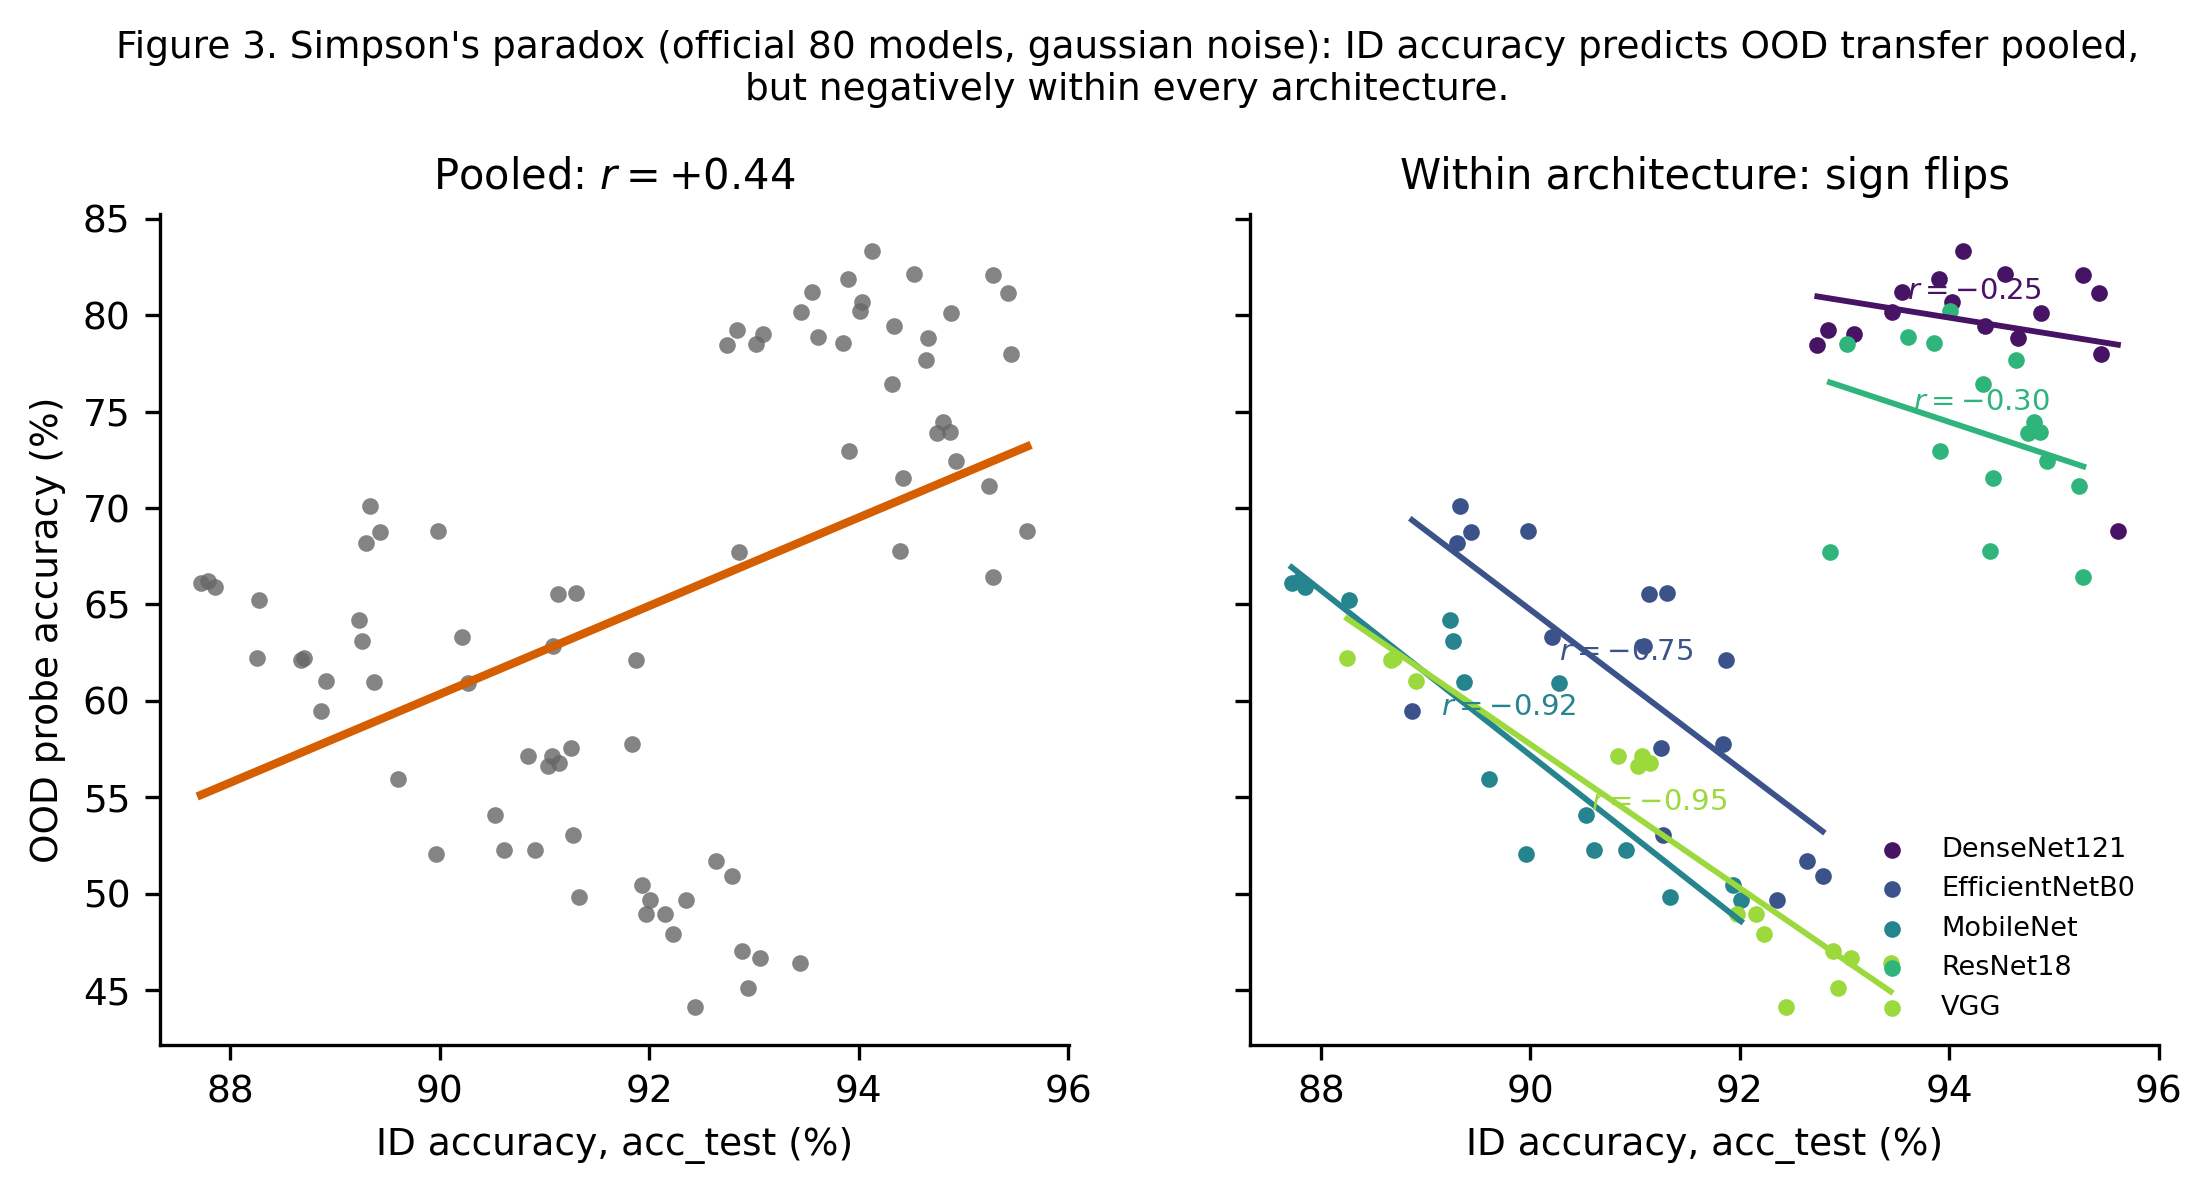
\includegraphics[width=\linewidth]{figures/fig3_simpson.png}
\caption{Simpson's paradox on the official 80-model release (gaussian noise scenario). Left: pooled over all models, ID accuracy is positively associated with OOD transfer. Right: the same association computed within each architecture, where every coefficient is negative.}
\label{fig:simpson}
\end{figure}

\subsection{Band sensitivity}
\label{sub:bandsens}

Residualized $D_{\mathrm{eff}}$ stays within [+0.71, +0.78] across $b \in \{1,2,3,5\}$pp on the 80-model release, and within [+0.89, +0.93] on the 224-model release. The baseline's residualized coefficient moves between +0.39 and +0.57 on the 224 release and between $-0.61$ and $-0.77$ on the 80-model release across the same bands --- stable within each dataset, opposite across datasets. (The one band at which the 80-model baseline reaches $-0.61$ is $b=2.5$pp; the range is otherwise $-0.63$ to $-0.77$. A band of 8pp would be degenerate --- it retains all 80 models and is the unmatched sample --- so it is not reported as a sensitivity point.)

\begin{figure}[t]
\centering
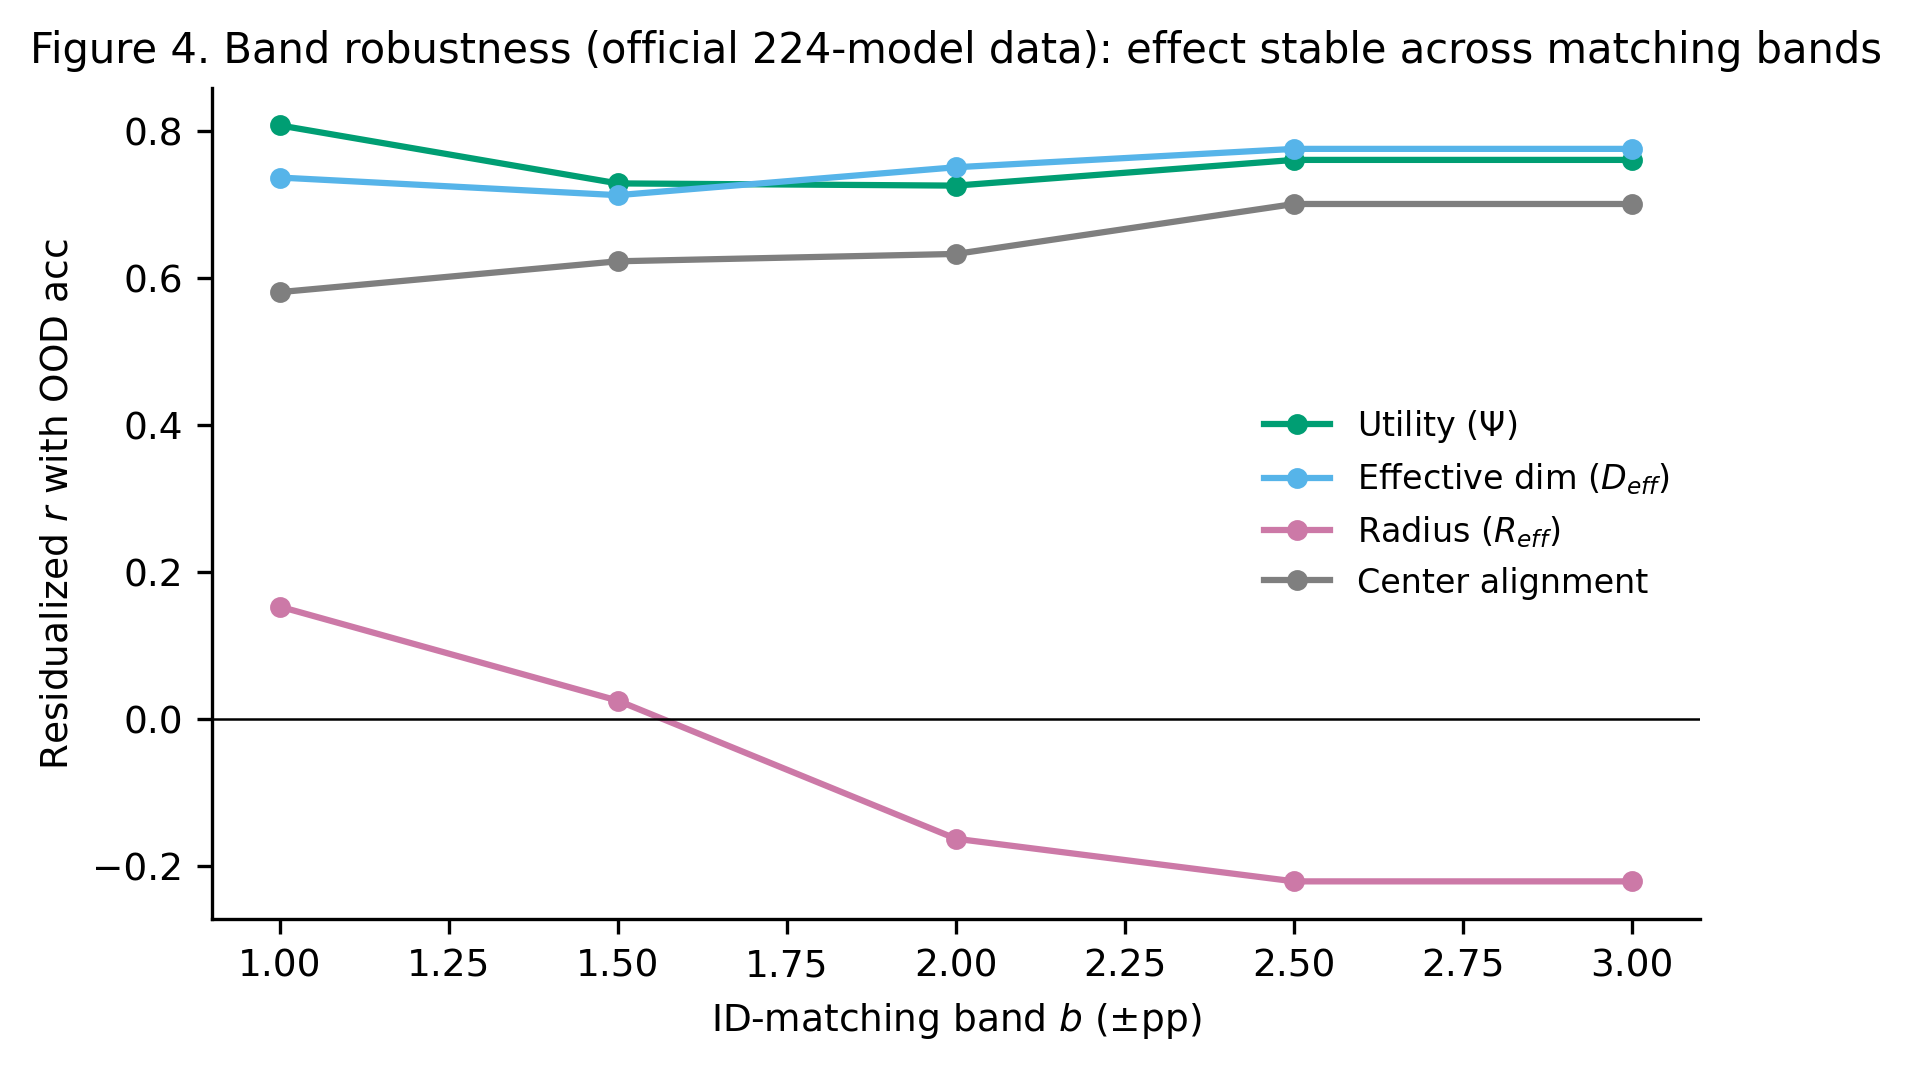
\includegraphics[width=0.85\linewidth]{figures/fig4_band.png}
\caption{Band robustness on the official 224-model release: the residualized correlation of the GLUE markers with OOD accuracy is stable across ID-matching bands $b$.}
\label{fig:band}
\end{figure}

\subsection{Bootstrap confidence intervals}\label{sec:signinstability}
\label{sub:bootstrap}

Stratified bootstrap over the full pipeline (2000 replicates; re-selection of the ID-matched subset, refit of residualization, both statistics recomputed):

\begin{table}[t]
\caption{Stratified bootstrap 95\% confidence intervals for the residualized correlation with OOD accuracy, together with the per-marker robustness rate.}
\label{tab:bootstrap}
\centering
\small
\setlength{\tabcolsep}{6pt}
\begin{tabular}{@{}p{2.6cm}p{3.3cm}p{3.6cm}p{3.4cm}@{}}
\hline
Quantity & Dataset & 95\% CI (resid.\ $r$) & Bootstrap robust rate \\
\hline
$D_{\mathrm{eff}}$ & 224 models & \textbf{[+0.879, +0.955]} & 100\% \\
\hline
$\Psi_{\mathrm{eff}}$ & 224 models & \textbf{[+0.842, +0.938]} & 100\% \\
\hline
$D_{\mathrm{eff}}$ & 80 models & [+0.581, +0.833] & 100\% \\
\hline
numerical rank & ours (48, all) & [+0.797, +0.923] & 100\% \\
\hline
numerical rank & ours (36, converged) & [+0.819, +0.943] & 100\% \\
\hline
\textbf{ID accuracy} & 224 models & \textbf{[+0.215, +0.622]} & 13\% \\
\hline
\textbf{ID accuracy} & 80 models & \textbf{[$-$0.825, $-$0.417]} & 80\% \\
\hline
\textbf{ID accuracy} & ours (48, all) & \textbf{[$-$0.659, $-$0.181]} & 23\% \\
\hline
\textbf{ID accuracy} & ours (36, converged) & \textbf{[$-$0.803, $-$0.420]} & 0\% \\
\hline
\end{tabular}
\end{table}

The two official releases yield baseline intervals that each exclude zero --- in opposite directions, with no overlap. Within any single dataset, ID accuracy looks like a significant predictor; across populations, its sign does not transfer. This is a stronger negative than ``the markers beat the baseline'': at fixed ID matching, the baseline is not a stable quantity whose value can be taken for granted. (Both releases use the same OOD target --- the CIFAR-100 linear probe --- and share no models; we verified that the OOD column is identical across the six corruption scenarios within the second release, so the two intervals are computed on the same quantity.) The bootstrap robust rate column makes the same point from a second angle: $D_{\mathrm{eff}}$ passes the rank criterion in every replicate on both official releases, while the baseline passes it in 13\% and 80\% respectively. On our own models the baseline's robust rate is 23\% over all 48 and 0\% over the converged 36.

\subsection{Shift-type decomposition}
\label{sub:shifttype}

On the 80-model, six-corruption release, predicting corruption accuracy:

We report \textbf{both} an uncontrolled (pooled) Spearman $\rho$ and the Protocol-A coefficient (C1 ID-matching at $\pm2$pp + C2 architecture residualization), so that the shift-type conclusion can be checked against the same instrument used everywhere else in this paper. The two columns agree on every qualitative claim; they differ in magnitude, and in one case in sign.

\begin{table}[t]
\caption{Shift-type decomposition on the 80-model release: pooled and Protocol-A coefficients for six corruption scenarios.}
\label{tab:shifttype}
\centering
\scriptsize
\setlength{\tabcolsep}{2.5pt}
\begin{tabular}{@{}p{2.10cm}p{1.85cm}p{0.85cm}p{1.15cm}p{0.95cm}p{2.15cm}p{1.25cm}p{1.60cm}p{0.95cm}@{}}
\hline
Scenario & Best predictor (pooled) & $\rho$ & ID-acc $\rho$ & ID-acc rank & Best predictor (Protocol A) & $\rho_{\text{resid}}$ & ID-acc $\rho_{\text{resid}}$ & ID-acc rank \\
\hline
fog & ID accuracy & $+0.987$ & $+0.987$ & 1/12 & ID accuracy & $+0.918$ & $+0.918$ & 1/12 \\
\hline
brightness & ID accuracy & $+0.994$ & $+0.994$ & 1/12 & ID accuracy & $+0.968$ & $+0.968$ & 1/12 \\
\hline
contrast & ID accuracy & $+0.965$ & $+0.965$ & 1/12 & ID accuracy & $+0.772$ & $+0.772$ & 1/12 \\
\hline
gaussian\_\allowbreak noise & mean angle & $-0.666$ & $+0.182$ & 7/12 & sparsity & $+0.297$ & $-0.087$ & 8/12 \\
\hline
pixelate & center alignment & $-0.451$ & $-0.122$ & 10/12 & sparsity & $+0.515$ & $+0.215$ & 6/12 \\
\hline
jpeg\_\allowbreak compression & center alignment & $-0.382$ & $+0.122$ & 10/12 & sparsity & $+0.602$ & $-0.010$ & 11/12 \\
\hline
\end{tabular}
\end{table}

Under photometric and structural corruptions, ID accuracy is essentially a sufficient statistic: it is the single best predictor under \textbf{both} instruments ($+0.92$ to $+0.97$ under Protocol A, ranked 1st of 12). Under noise and compression corruptions it collapses --- under Protocol A its coefficient falls to $-0.09$ to $+0.22$ and its rank drops to 6th--11th of 12, and the best marker in every one of these three scenarios is \emph{sparsity}, whose sign differs by scenario ($+0.30$ for gaussian noise, $+0.52$ for pixelate, $+0.60$ for jpeg compression).

The two instruments do not agree in sign everywhere, and that is itself informative: \texttt{pixelate} moves from $-0.12$ (pooled) to $+0.22$ (Protocol A) for the baseline, and its best marker changes from center alignment to sparsity. A shift-type claim stated on pooled correlations alone would therefore be measuring the confound, not the phenomenon. We report the controlled column as primary and the pooled column for reference; the split into two regimes survives either way, which is the claim we make.

The original study's aggregate statement about corruptions conflates these two regimes. Our 19-scenario replication on self-trained models reproduces the split. Ranking ID accuracy against the seven publicly computable markers for each scenario: ID accuracy ranks 1st of 8 in 11 of the 19 scenarios (brightness, fog, frost, saturate, snow, spatter, defocus blur, elastic transform, gaussian blur is 2nd, motion blur, zoom blur, jpeg compression) and ranks 7th--8th of 8 in the four noise scenarios (gaussian noise 8th, shot noise 8th, impulse noise 7th, speckle noise 7th) and in pixelate (7th) and glass blur (8th). One photometric scenario is an exception in our models: \emph{contrast}, where ID accuracy ranks 7th of 8 ($\rho=+0.09$), in contrast to the official 80-model release where it is the strongest predictor ($\rho=+0.97$). We report this exception rather than average it away: contrast is precisely the case where the two datasets disagree, and it is the clearest indication in our data that the corruption taxonomy is not as clean as a two-way split suggests.

\begin{figure}[t]
\centering
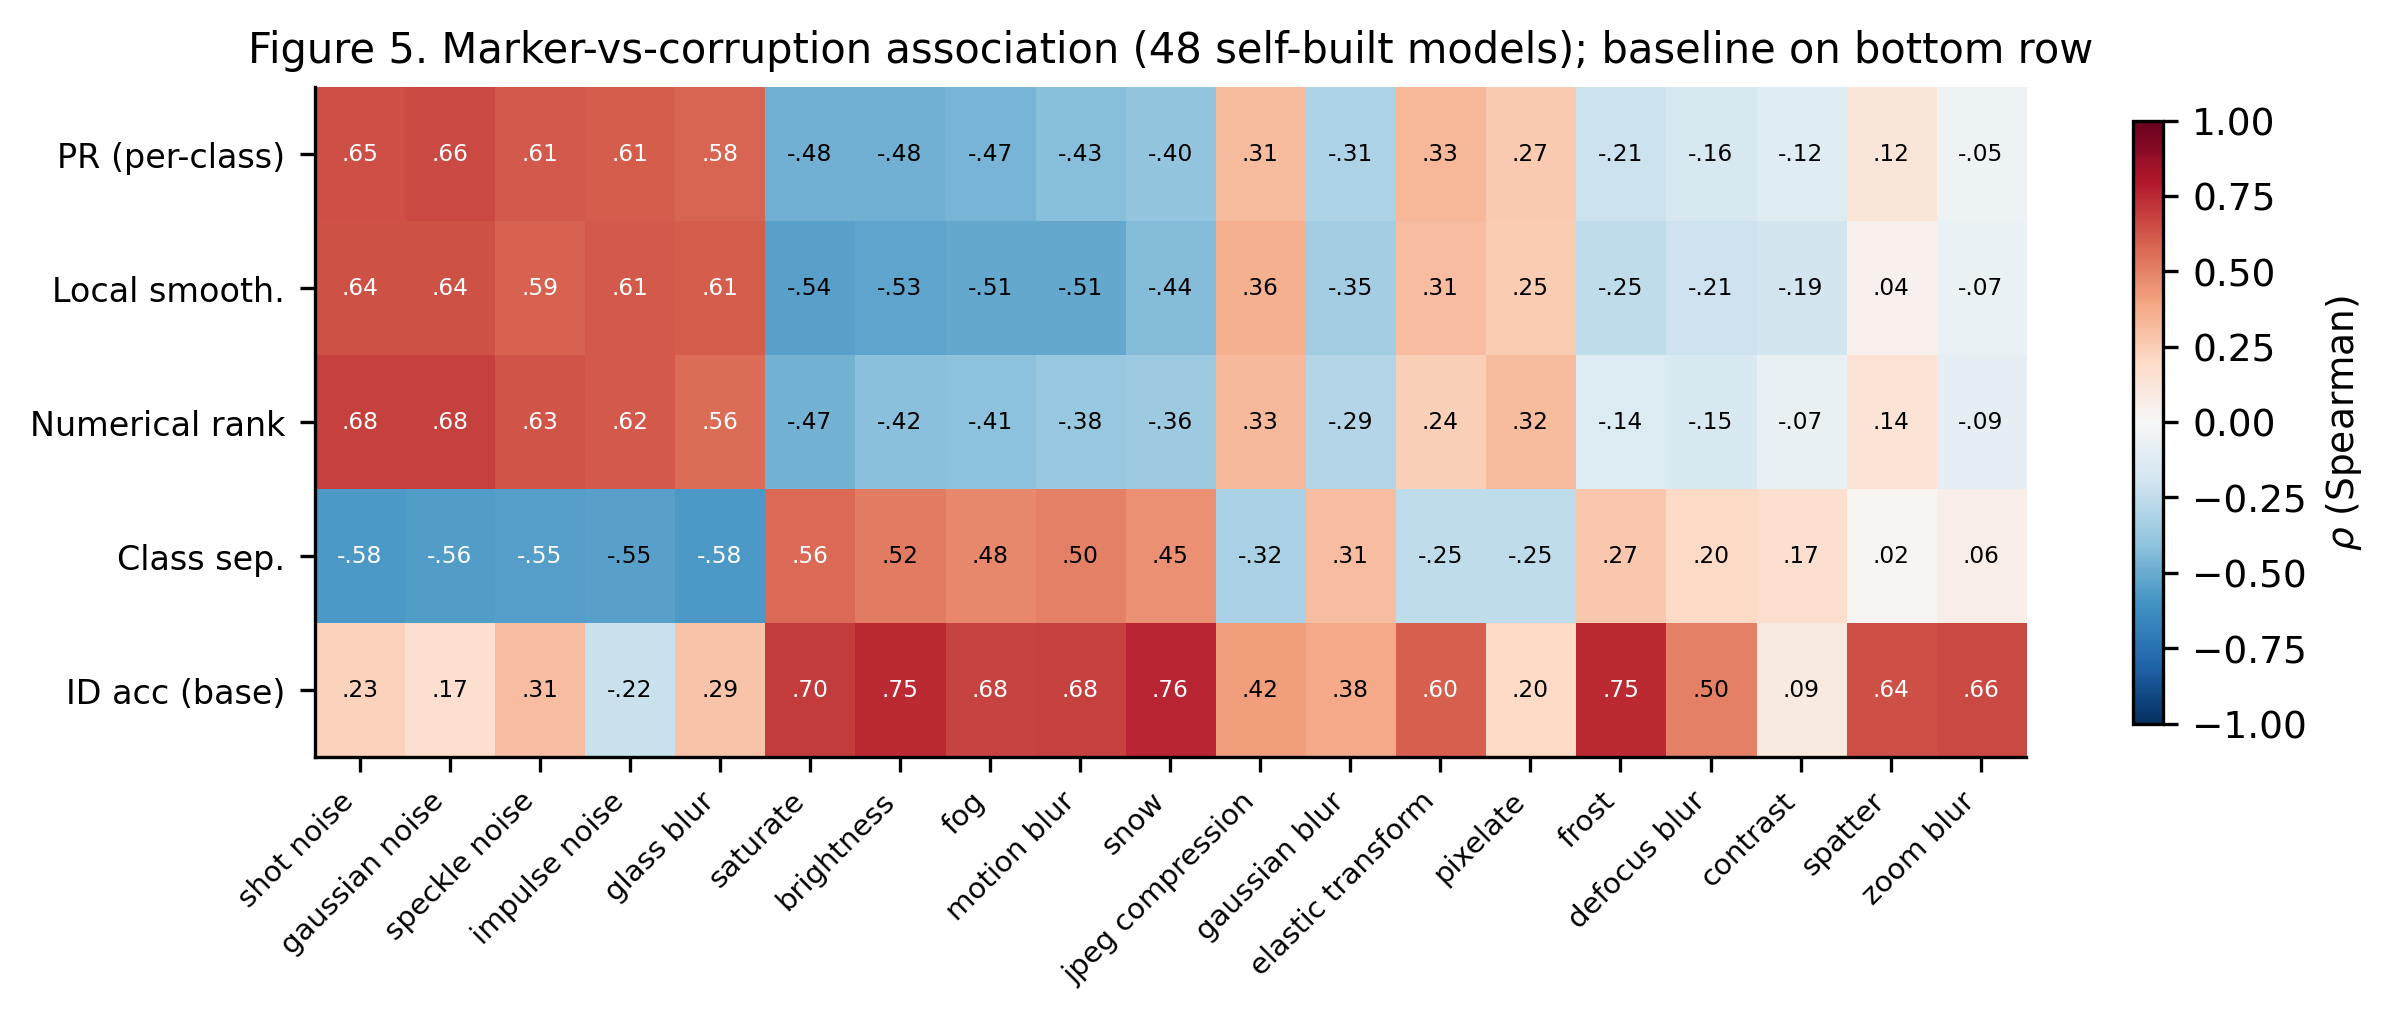
\includegraphics[width=\linewidth]{figures/fig5_corruption.png}
\caption{Marker-versus-corruption association on the 48 self-trained models. The bottom row is the ID-accuracy baseline; photometric and structural corruptions are predicted well by ID accuracy, whereas noise and compression scenarios are not.}
\label{fig:corruption}
\end{figure}

\subsection{Independent replication: two class-level shifts}
\label{sub:replication}

On our 48 ResNet-18 models (grouping variable: learning-rate family), residualized coefficients under ID matching at $\pm2$pp:

\begin{table}[t]
\caption{Independent replication on 48 self-trained ResNet-18 models: residualized correlations with two class-level shifts under ID matching at $\pm2$pp.}
\label{tab:replication}
\centering
\small
\setlength{\tabcolsep}{6pt}
\begin{tabular}{@{}p{4.6cm}p{3.4cm}p{3.4cm}@{}}
\hline
Predictor & CIFAR-100 & Tiny-ImageNet \\
\hline
numerical rank & \textbf{$+0.870$} & \textbf{$+0.853$} \\
\hline
local smoothness & $+0.832$ & $+0.792$ \\
\hline
participation ratio & $+0.701$ & $+0.707$ \\
\hline
self-impl.\ GLUE dim (relative only) & --- & $+0.729$ \\
\hline
\textbf{ID accuracy} & \textbf{$-0.439$} ($p$=0.002) & \textbf{$-0.338$} ($p$=0.022) \\
\hline
\end{tabular}
\end{table}

\textbf{The baseline does not replicate as a uniformly negative sign --- it replicates as an unstable sign.} Applying condition C4 to the baseline itself (per-family coefficients within each learning-rate family) shows that the aggregate negative coefficient conceals a sign flip. In the table below, each family is residualized within itself on the ID-matched subset (C1 applied at the population level, C2 applied within family); the family-wise ID-matching center differs from the one used in the converged-family sensitivity analysis below, so the two tables can differ slightly for the same family.

\begin{table}[t]
\caption{Per-learning-rate-family coefficients for the ID-accuracy baseline (condition C4) on the 48 self-trained models.}
\label{tab:families}
\centering
\small
\setlength{\tabcolsep}{6pt}
\begin{tabular}{@{}p{2.8cm}p{1.2cm}p{3.6cm}p{3.2cm}@{}}
\hline
lr family & $n$ & CIFAR-100 resid.\ $r$ & Tiny resid.\ $r$ \\
\hline
0.125 & 12 & $-0.802$ & $-0.739$ \\
\hline
0.25 & 11 & $-0.603$ & $-0.134$ \\
\hline
0.5 & 12 & $-0.330$ & $-0.186$ \\
\hline
1.0 & 11 & \textbf{$+0.694$} & \textbf{$+0.415$} \\
\hline
\textbf{C4 sign-consistent?} & & \textbf{No} & \textbf{No} \\
\hline
\end{tabular}
\end{table}

The $lr=1.0$ family is not a converged subpopulation: its OOD range is 7.1--14.7\%, against 13.7--32.4\% for the other three, and its models sit in a low-transfer training regime rather than a comparable one. Restricting to the three converged families (36 models, $n=34$ after ID matching) leaves the baseline negative in all three ($r=-0.97/-0.60/-0.33$) and strengthens the aggregate to \textbf{$-0.658$} (CIFAR-100) and \textbf{$-0.513$} (Tiny-ImageNet), with bootstrap 95\% CIs $[-0.80,-0.42]$ and $[-0.70,-0.22]$ (probability of a positive coefficient $\approx 0$\%). Geometric markers are unchanged or strengthened under this restriction (numerical rank $+0.892/+0.884$, bootstrap robustness 100\%).

We therefore report the baseline's behaviour as \textbf{sign instability rather than a replicated negative sign}. Both readings support the same conclusion --- the baseline is not a stable reference point --- but the instability is the more accurate description, and it is the one our own protocol's sign-consistency condition detects rather than excuses.

\begin{figure}[t]
\centering
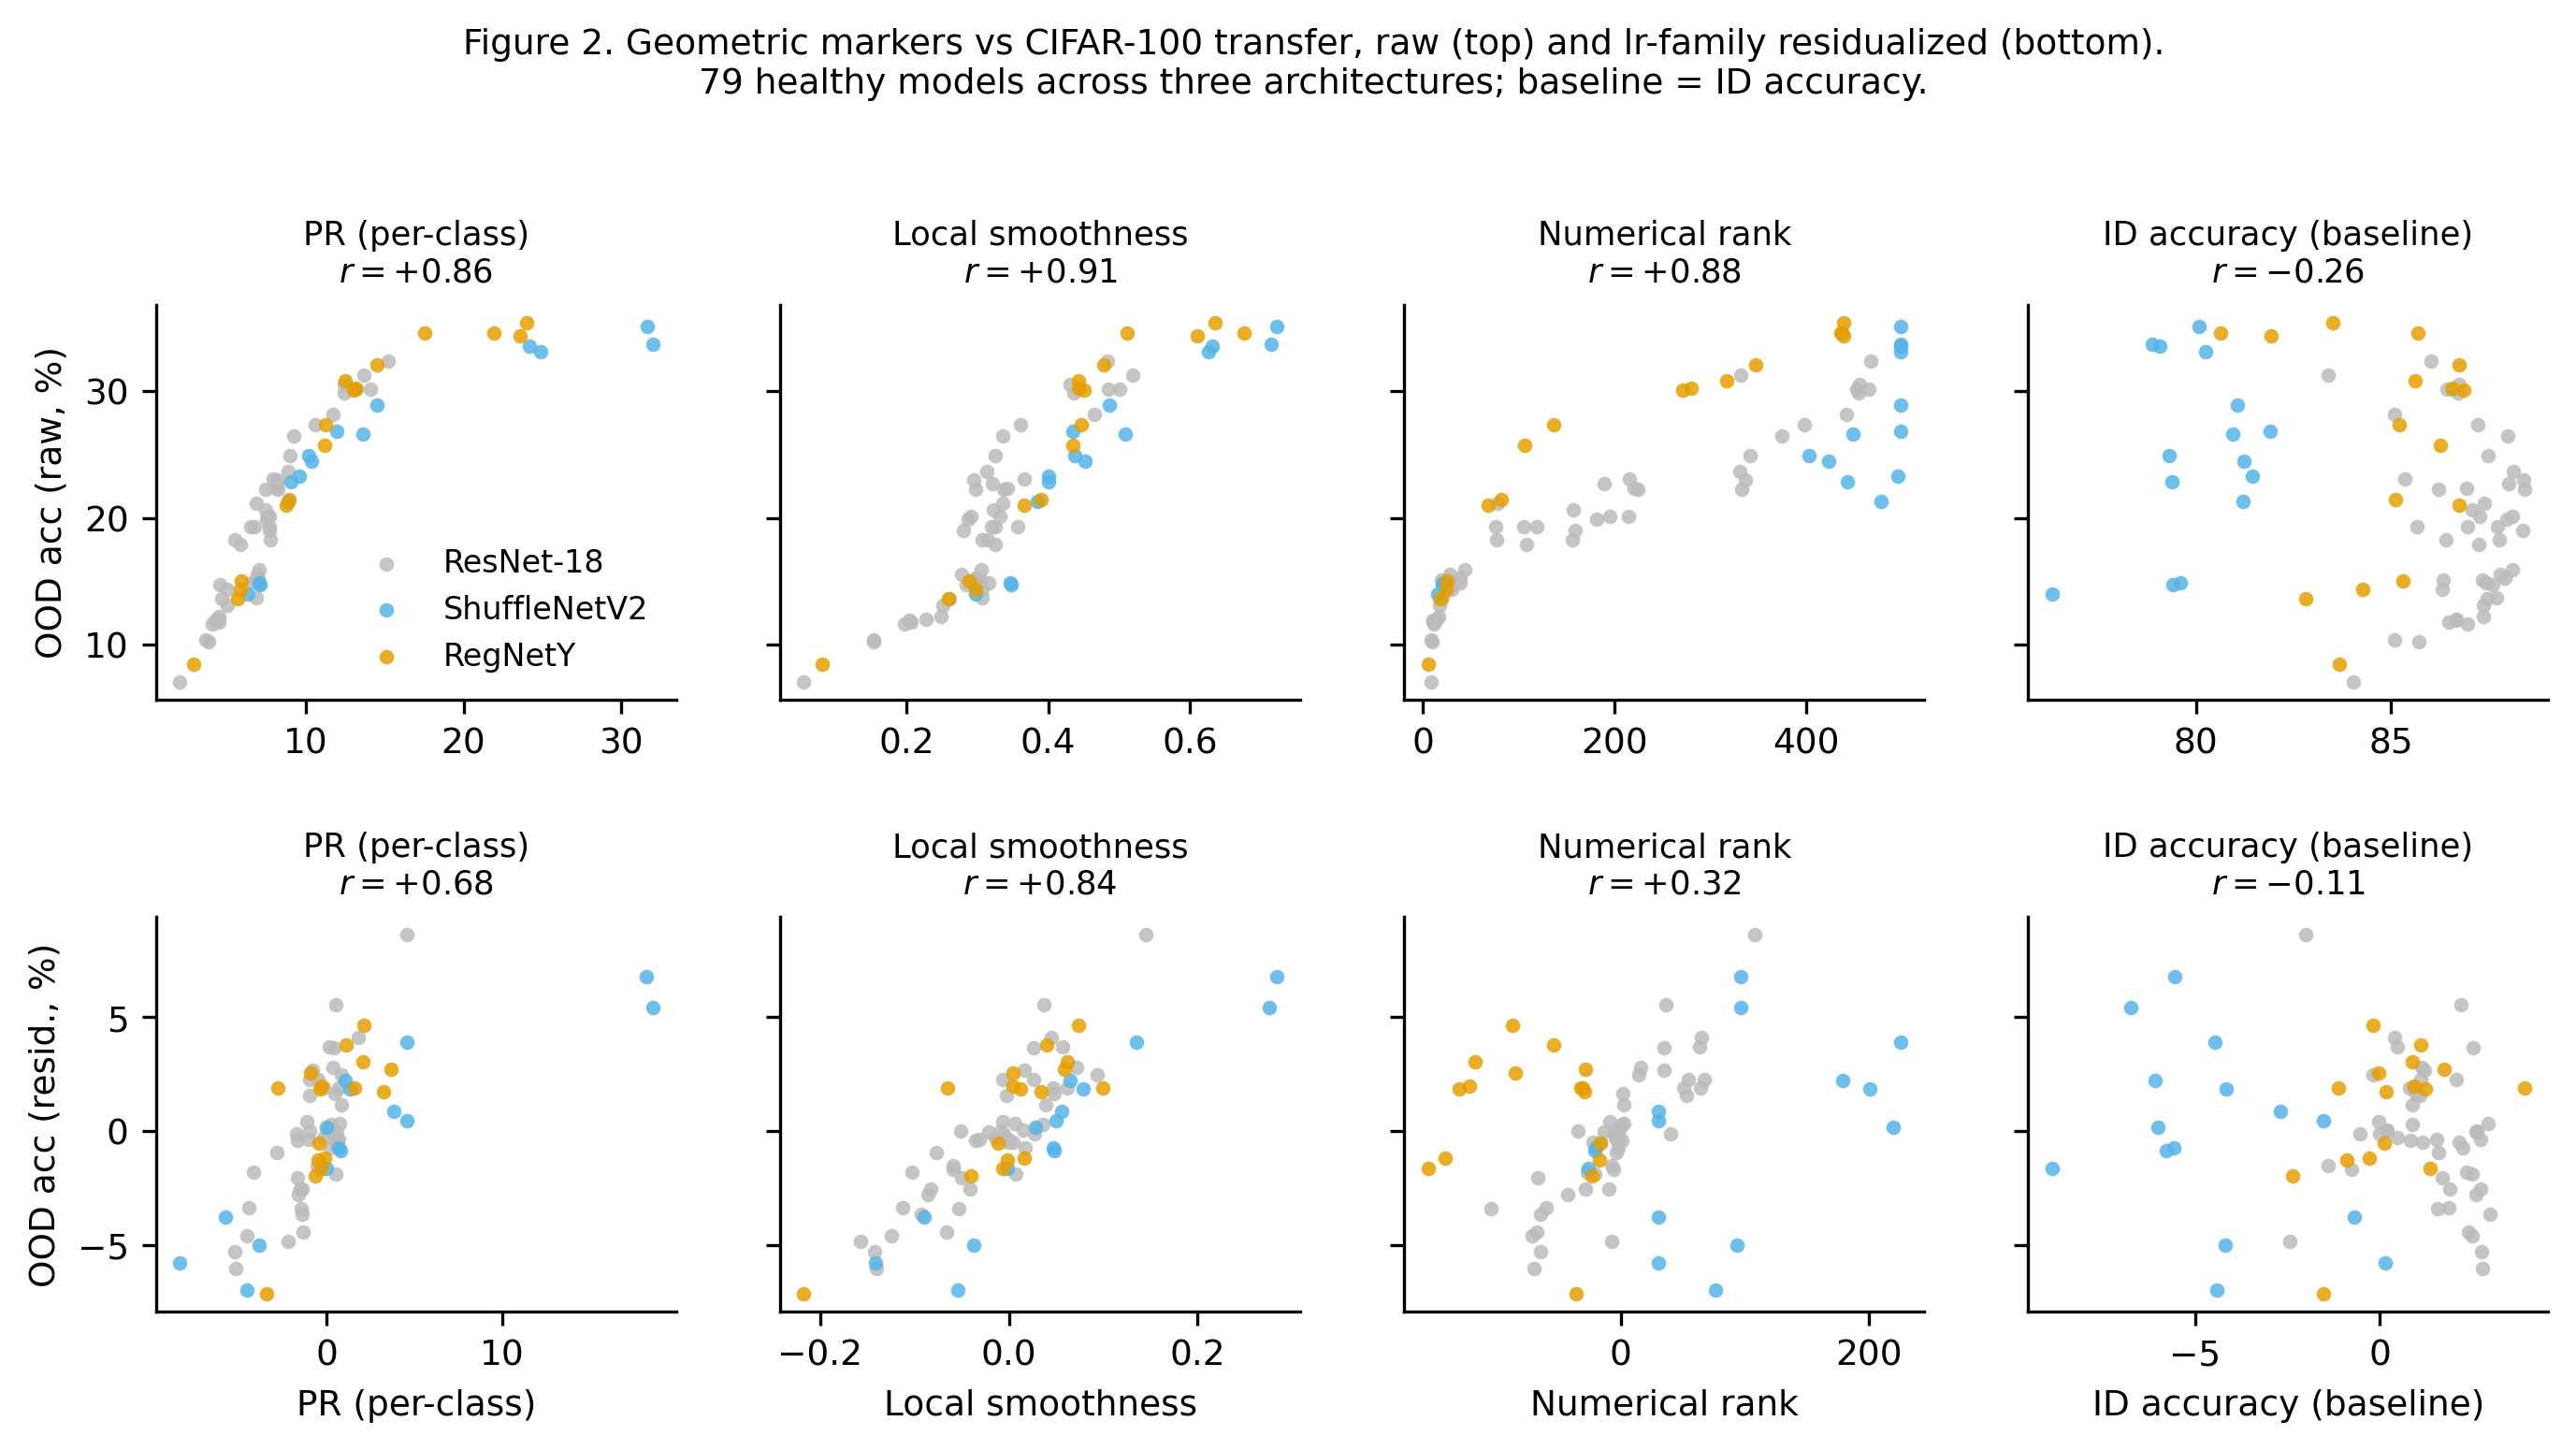
\includegraphics[width=\linewidth]{figures/fig2_scatter.png}
\caption{Geometric markers versus CIFAR-100 transfer on the 79 healthy self-trained models across three architectures. Top row: raw values. Bottom row: learning-rate-family residualized. In both rows the geometric markers track transfer while the ID-accuracy baseline does not.}
\label{fig:scatter}
\end{figure}

\begin{figure}[t]
\centering
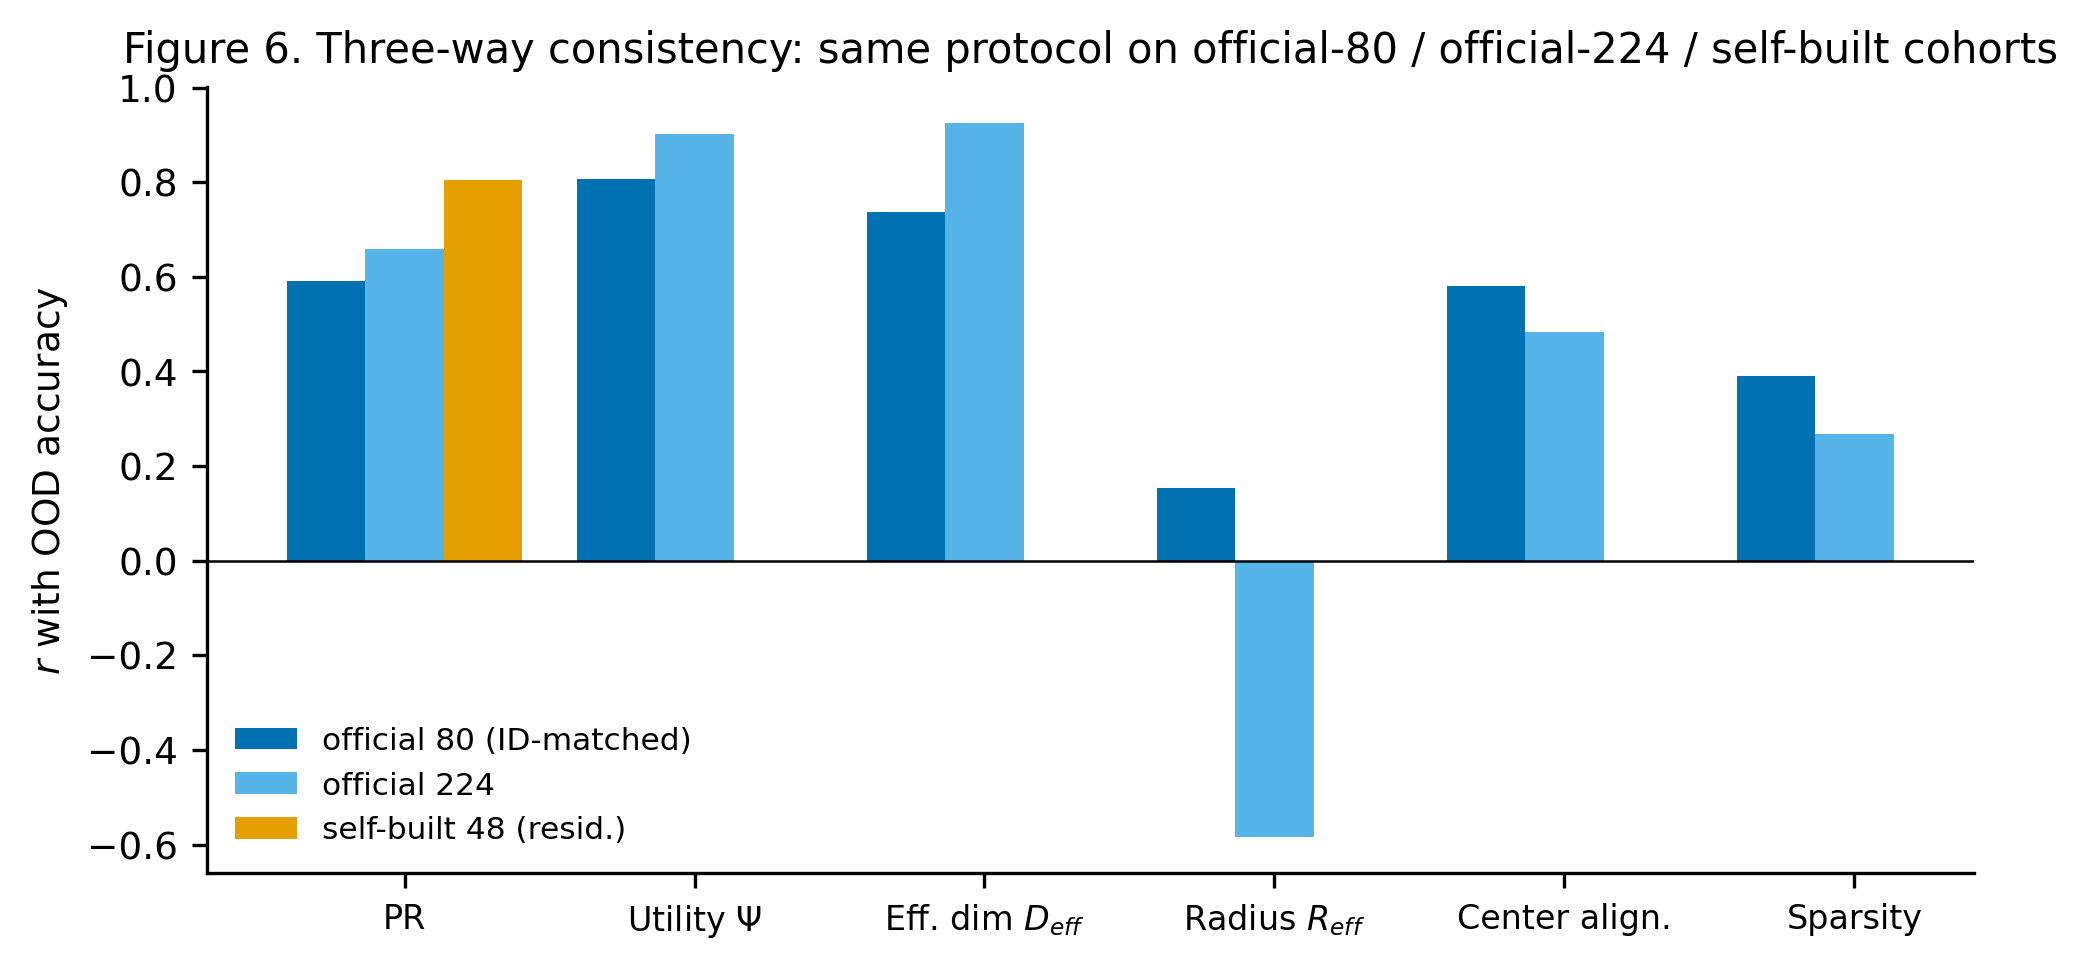
\includegraphics[width=0.9\linewidth]{figures/fig6_threeway.png}
\caption{Three-way consistency of the protocol across cohorts: the official 80-model and 224-model releases and the self-trained 48-model cohort, evaluated with the same protocol and the same marker set.}
\label{fig:threeway}
\end{figure}

\subsubsection{Cross-architecture replication}
\label{subs:crossarch}

Adding ShuffleNetV2 and RegNetY (79 healthy models out of 80 trained; grouping variable: architecture):

\emph{Cross-architecture subset} ($\pm2$pp around the pooled mean; $n=36$): participation ratio $+0.941$ / $+0.948$ ($\rho=+0.982$ / $+0.981$), local smoothness $+0.956$ / $+0.930$, numerical rank $+0.943$ / $+0.952$ --- all with consistent per-architecture signs; ID accuracy $+0.153$ ($p=0.37$) / $+0.145$ ($p=0.40$) with split signs. OOD span preserved: 100\% (CIFAR-100), 93\% (Tiny-ImageNet) at an ID span of 3.7pp.

\emph{Within-architecture protocol} (each architecture matched at its own mean; C2 residualization is applied over \emph{learning-rate families} within the architecture, which is the nuisance dimension that varies inside any single architecture):

\begin{table}[t]
\caption{Within-architecture protocol: residualized correlations by architecture for two class-level shifts. Each architecture is ID-matched around its own mean, and C2 residualization removes learning-rate-family main effects within that architecture (the nuisance dimension that varies inside any single architecture).}
\label{tab:withinarch}
\centering
\small
\setlength{\tabcolsep}{6pt}
\begin{tabular}{@{}p{2.8cm}p{2.6cm}p{4.4cm}p{4.4cm}@{}}
\hline
Arch & shift & PR resid.\ $r$ & ID-acc resid.\ $r$ \\
\hline
ResNet-18 & C100 / Tiny & $+0.701$ / $+0.707$ & $-0.439$ / $-0.338$ \\
\hline
ShuffleNetV2 & C100 / Tiny & \textbf{$+0.988$ / $+0.985$} & \textbf{$-0.637$ / $-0.584$} \\
\hline
RegNetY & C100 / Tiny & $+0.659$ (p=.014) / $+0.536$ (p=.059) & $+0.053$ (n.s.) / $-0.019$ (n.s.) \\
\hline
\end{tabular}
\end{table}

Across three architectures and two shifts (six cells), the baseline is significantly positive in none, significantly negative in four, and null in two (small $n$). Geometric markers are significant and positive in five of six cells (0.54--0.99), strongest for ShuffleNetV2 (+0.99).

One structural observation, and a limit of the protocol itself. ShuffleNetV2's ID-accuracy ceiling (82\%) falls below the pooled mean band (83.2--87.2\%), so an ID-matched selection \emph{centered on the pooled mean} excludes the entire architecture. We state this plainly as a limitation of C1 rather than as a finding: conditioning on ID accuracy is exactly what C1 prescribes, and any selection that uses ID accuracy will, by construction, exclude population segments whose ID accuracy is outlying --- here, a low-capacity family. This is a self-reference the protocol cannot dissolve, and it is worth naming because ID-matched selection is not neutral with respect to the baseline it is meant to control. Our remedy is the within-architecture protocol reported above, in which each architecture is matched around \emph{its own} mean and no family is excluded; under that protocol ShuffleNetV2 is present, and its markers are the strongest we measure ($+0.99$), with the baseline most negative ($-0.64$). A reader who prefers a band centered on each group's own mean throughout obtains the same qualitative conclusions with more groups represented.

\subsubsection{Cross-implementation check (ordering, not value)}
\label{subs:crossimpl}

Our independent implementation of the GLUE dimension --- used strictly for relative comparisons (\srcref{sub:datasources}) --- correlates with OOD accuracy at $r=+0.91$ ($\rho=+0.92$) on our 48 models, against $+0.87$ ($\rho=+0.87$) for the released implementation on the official ResNet-18 subset ($n=41$, ID-matched at $\pm1$pp). Different implementation, different data, same ordering strength. The same check shows $R_{\mathrm{eff}}$ and $\Psi_{\mathrm{eff}}$ do not transfer across implementations, consistent with their sign instability across releases (\srcref{sub:bootstrap}).

\subsubsection{Geometric markers and ID accuracy carry near-orthogonal information}
\label{subs:orthogonal}

The results above establish that geometric markers predict class-level transfer well and that ID accuracy does not. A stronger, mechanism-level reading is available on our 48 self-trained models: \textbf{the two quantities are close to statistically independent of each other}, and this is why one cannot substitute for the other.

\begin{table}[t]
\caption{Near-orthogonality of geometric markers and ID accuracy on the 48 self-trained models, with the partial correlation controlling for ID accuracy.}
\label{tab:orthogonal}
\centering
\small
\setlength{\tabcolsep}{4pt}
\begin{tabular}{@{}p{3.3cm}p{2.1cm}p{2.2cm}p{2.3cm}p{4.1cm}@{}}
\hline
Marker & vs.\ ID accuracy & vs.\ CIFAR-100 & vs.\ Tiny-ImageNet & partial $r$ with CIFAR-100, controlling ID accuracy \\
\hline
self-impl.\ GLUE dimension & \textbf{$-0.170$} & $+0.908$ & $+0.919$ & $+0.686$ \\
\hline
participation ratio & \textbf{$-0.074$} & $+0.951$ & $+0.945$ & $+0.756$ \\
\hline
numerical rank & \textbf{$-0.044$} & $+0.944$ & $+0.949$ & $+0.849$ \\
\hline
local smoothness & \textbf{$-0.090$} & $+0.899$ & $+0.878$ & $+0.861$ \\
\hline
\textbf{ID accuracy (baseline)} & $+1.000$ & $-0.045$ & $-0.027$ & --- \\
\hline
\end{tabular}
\end{table}

Every geometric marker is essentially uncorrelated with ID accuracy on this population ($-0.17$ to $-0.04$) while correlating at $+0.90$ to $+0.95$ with OOD accuracy; ID accuracy shows the mirror image ($-0.05$ with CIFAR-100, $-0.03$ with Tiny-ImageNet). Crucially, the association survives conditioning: after removing the linear component of ID accuracy, the markers retain partial correlations of $+0.69$ to $+0.86$ with CIFAR-100 transfer. (The first three columns are raw correlations on all 48 models; the last is a partial correlation computed on learning-rate-residualized variables with the linear component of ID accuracy removed from both sides.)

This is a third, independent line of evidence for the paper's central claim, and unlike the cross-release comparison of \srcref{sub:bootstrap} it requires no assumption about the comparability of two released datasets, no ID-matching band, and no bootstrap. The mechanism it suggests is straightforward: \textbf{ID accuracy and representational geometry are measuring different things} --- how well the network fits the training distribution versus how the learned representation is organised. On class-level shifts, only the second is informative. A reader who wants a single sentence of the paper's thesis can take this one: at fixed training task, the two candidate signals are nearly independent, and only one of them tracks out-of-distribution transfer.

\section{Discussion}
\label{sec:discussion}

\textbf{What the original study got right.} The geometric markers are real: under the strictest controls we can construct --- ID matched, architecture residualized, rank-consistent, sign-consistent, bootstrap-confirmed at 100\% robustness --- $D_{\mathrm{eff}}$ and $\Psi_{\mathrm{eff}}$ retain associations with OOD accuracy of +0.90 to +0.93. Nothing in this paper should be read as doubting the markers themselves.

\textbf{What the comparison missed.} The ``markers beat ID accuracy'' framing is not wrong but underdetermined, because ID accuracy is not a fixed reference point. Its association with OOD transfer, at fixed ID matching and with architecture effects removed, changes sign between populations --- and within our own model population it even changes sign across training families. Three specific mechanisms:

\begin{enumerate}
\item \emph{Architecture capacity sorting.} Within the ID-matched band, remaining ID-accuracy variation mostly reflects architecture capacity allocation, which anti-correlates with transfer in this regime: compact well-trained architectures (ResNet18, DenseNet121) land slightly lower on ID but transfer better; higher-ID VGG/MobileNet variants transfer worse. The pooled positive coefficient is a between-family artifact.
\item \emph{Population dependence, not a fixed weakness.} On one release the baseline is positive, on another negative, and in our own models it is negative in aggregate but positive in one learning-rate family. This is not evidence that accuracy is a bad predictor in general --- it is evidence that its coefficient is a property of the population being modelled, and therefore cannot be treated as a fixed yardstick.
\item \emph{Shift-type dependence.} Under photometric/structural corruptions, ID accuracy is genuinely a near-sufficient statistic ($\rho_{\text{resid}}\approx0.77$--$0.97$); under noise/compression it is noise. A single aggregate statement about ``corruption robustness'' averages over two opposite regimes.
\item \emph{The two signals measure different things.} On our own models, geometry and accuracy are nearly uncorrelated with each other ($-0.17$ to $-0.04$). This is the mechanistic reason the baseline cannot serve as a stand-in: it is not a noisy version of the marker, it is a different quantity. A diagnostic that is nearly orthogonal to the cheap test is exactly the kind worth having --- and this is where a geometric marker earns its cost.
\end{enumerate}

\textbf{A self-reference we cannot dissolve.} Our own C1 conditions on ID accuracy, and we then argue that ID-accuracy-based comparisons are unstable. A reader may reasonably observe that the protocol inherits the very quantity it is auditing. We think this is the right trade for a different reason than the original framing: without ID matching, the comparison is confounded by between-architecture differences, and the confound is demonstrably larger than the effect being compared (pooled $r=+0.48$ on one release versus $-0.63$ under matching). The honest position is that C1 is a \emph{choice}, not a neutral operation, and that its known consequence --- excluding population segments with outlying ID accuracy --- must be reported alongside the result. We do so in \srcref{subs:crossarch}, and we provide the within-architecture variant in which no family is excluded.

\textbf{Why the negative baseline is not paradoxical.} At fixed ID accuracy, the marginal ID point is not ``a slightly better model'' but ``a model that spent its capacity differently'' --- and in this population that allocation trades against transfer. The negative sign is what an architecture-capacity tradeoff looks like from inside an ID-matched window; it is not a claim that lower ID accuracy causes better transfer.

\textbf{Implications for practitioners.}
\begin{itemize}
\item Do not use geometric markers for in-distribution model selection; at fixed task and shift-free evaluation they carry little or no information (our Phase-0 experiment found no nontrivial marker with in-cluster validity --- see supplementary).
\item For cross-architecture OOD comparison, ID accuracy is not a usable baseline; report markers alongside, with the four-condition protocol.
\item Match the marker to the shift: photometric/structural corruptions admit ID accuracy; noise, compression, and class-level shifts require geometric (or other) markers.
\end{itemize}

\textbf{On which markers to trust.} Across everything we ran, $D_{\mathrm{eff}}$ is the only marker that passes all conditions on every dataset, implementation, and architecture; $\Psi_{\mathrm{eff}}$ on all but the cross-implementation check; participation ratio and numerical rank are strong within-architecture but lose cross-architecture sign consistency on the official releases (though they regain it on ours --- a discrepancy we flag rather than resolve). $R_{\mathrm{eff}}$ and ID accuracy fail sign stability across releases.

\textbf{Relation to the brain--AI program.} This project began from the hypothesis that representational ``elegance'' could serve as a universal quality measure for networks, in the spirit of the brain--AI correspondence literature. The result is more specific and more useful: geometric markers are \emph{conditional} instruments. They are powerful exactly where accuracy-based selection fails (distribution shift, cross-architecture comparison) and powerless where it works (in-distribution). A biomarker analogy fits: a diagnostic is valuable precisely when it disagrees with the cheap test in a controlled way --- not when it replaces it everywhere.

\section{Limitations}
\label{sec:limitations}

\begin{enumerate}
\item \textbf{Shared model population across corruption scenarios.} The six corruption scenarios in the 80-model release share one set of models and one set of ID-side markers; only the corruption-side labels differ. Corruption scenarios are therefore not independent samples of each other.
\item \textbf{Reliance on released measurements.} The primary analysis uses the original authors' released per-model values. Although public and auditable, conclusions about their method drawn from their own measurements warrant independent confirmation --- which \srcref{sub:replication} and \srcref{subs:crossarch} provide on separately trained models, and \srcref{sub:bootstrap} provides on their second release.
\item \textbf{Self-implementation of GLUE.} All headline values of $D_{\mathrm{eff}}$, $R_{\mathrm{eff}}$, $\Psi_{\mathrm{eff}}$ are the released ones. Our own implementation (public Algorithm 1 plus the anchor solver of \citet{chung2018classification}) reproduces the released PR and NC1 exactly, and the released radius within $\sim$10\%, but not the released dimension and utility; the appendix of the GLUE paper specifies per-pair analysis and Gaussianization preprocessing that our version does not cover, and no second reference checkpoint exists to cross-validate against. We therefore use our implementation only for ordering consistency (\srcref{subs:crossimpl}), never for absolute values.
\item \textbf{Class-level shift coverage.} Our replication side covers two class-level shifts (CIFAR-100, Tiny-ImageNet); the official side covers one. Neither covers full ImageNet-scale shift.
\item \textbf{Linear residualization.} Architecture adjustment uses dummy-variable OLS; interactions between architecture and hyperparameters are not modeled. Bootstrap intervals (\srcref{sub:bootstrap}) cover pipeline uncertainty under this linear adjustment but not specification uncertainty of the adjustment itself.
\item \textbf{Observational subset selection.} ID matching is a filter, not randomization; unmeasured confounders within the band cannot be excluded, though the band spans only 1.9--3.7 percentage points.
\item \textbf{Modern-architecture replication size.} ShuffleNetV2 and RegNetY contribute 15--16 models each (one lr-seed cell each diverged and was excluded). The within-architecture cells for RegNetY ($n=12$) are underpowered; its null baseline coefficients should be read as inconclusive rather than as evidence of no effect.
\item \label{lim:nonconverged} \textbf{A non-converged training regime in our own replication.} One learning-rate family in the 48-model collection ($lr=1.0$) does not reach a comparable OOD level (OOD 7.1--14.7\% against 13.7--32.4\% for the other three families). It is retained in the headline replication numbers --- where it produces the baseline's within-family sign flip and hence its instability --- and a converged-family sensitivity analysis excluding it is reported in \srcref{sub:replication}.
\item \label{lim:crossrelease} \textbf{Cross-release comparability rests on our own verification, not on the authors' confirmation.} The sign-instability result of \srcref{sub:bootstrap} compares two released datasets and assumes their \texttt{acc\_lp\_ood} columns were produced by the same probe pipeline. We verified independently that the two releases share no models and that the OOD column is constant across the six corruption scenarios of the second release, and the original study's appendix describes CIFAR-100 linear probing as the class-level OOD protocol in both cases. We could not verify the probe \emph{hyperparameters} (regularization, optimisation budget, feature layer) from the released files, which contain only resulting accuracies, and we have not obtained author confirmation. A difference in probe configuration between the two releases is an alternative explanation for the sign difference that we cannot exclude. Note that our main claim does not rest on this comparison: the near-orthogonality result of \srcref{subs:orthogonal} and the within-family sign flip of \srcref{sub:replication} are both established on data we generated ourselves, and they support the same conclusion without any cross-release assumption.
\item \textbf{Scope and modality.} All experiments are CIFAR-scale vision. Nothing here bears on language, audio, or larger scales, where capacity-allocation dynamics may differ.
\end{enumerate}

\section{Conclusion}
\label{sec:conclusion}

We re-examined the claim that representational-geometry markers outperform ID test accuracy as predictors of OOD generalization. Under a four-condition control protocol --- ID matching, confounder residualization, dual correlation statistics, cross-group sign consistency --- applied to the original study's own 224-model release, the task-relevant geometric markers survive intact ($D_{\mathrm{eff}}$: $r=+0.93$, $\rho=+0.85$, sign-consistent across all five architectures, 100\% bootstrap robustness). The baseline does not: at fixed ID accuracy and with architecture effects removed, the sign of the ID-accuracy association depends on the population --- positive on one release of the original study ($+0.39$, CI $[+0.22,+0.62]$), negative on another ($-0.63$, CI $[-0.83,-0.42]$), and, in our own models, negative in aggregate but flipping sign across training families. ``Markers versus accuracy'' is thus not a well-posed comparison unless the baseline's population-dependence is itself reported.

The markers' advantage is conditional. Under photometric and structural corruptions, ID accuracy is restored as a near-sufficient statistic; under noise, compression, and class-level shifts, it fails and geometry takes over. The two regimes were previously aggregated into one statement; separating them is, we think, the practically useful version of the original finding.

Everything replicates outside the original data: 78 self-trained models across three architectures (2015--2020 designs), two class-level shifts, an independent GLUE implementation used for ordering --- the baseline is significantly positive nowhere, and the geometric markers hold at 0.54--0.99 throughout, strongest on the more modern architectures. And on those same models the reason becomes explicit: geometric markers and ID accuracy are nearly orthogonal to each other ($-0.17$ to $-0.04$), with the markers correlating $+0.90$ to $+0.95$ with class-level transfer and the accuracy correlating $-0.05$. They were never measuring the same thing. Two structural findings deserve emphasis. First, an ID-accuracy-centered selection silently excludes low-capacity architectures whose ceiling falls below the matching band; we treat this as a limit of our own protocol and provide the within-architecture variant in which no family is excluded. Second, the protocol's sign-consistency condition, applied to the baseline rather than to the markers, is what reveals the instability --- the check that protects the markers' claim is the same check that destabilizes the comparison.

We release the protocol, all analysis code, and the 78 trained checkpoints. The protocol is not specific to geometry: any proposed cheap proxy for generalization --- logit statistics, activation sparsity, CKA variants --- should be able to pass through it before being compared to accuracy. The lesson of this exercise is narrower than ``geometry works'' and more durable: a proxy is valuable exactly where the cheap baseline fails, and demonstrating that requires controlling the baseline, not just beating it.

\section{Reproducibility statement}
\label{sec:repro}

All experiments use public data (CIFAR-10/100, CIFAR-10-C, Tiny-ImageNet) and public releases of the original study (MIT-licensed repository). The protocol implementation, the analysis code, the per-model measurements, and the 80 trained checkpoints are released at \href{https://github.com/zhouranxi/brainai-protocol-a}{github.com/zhouranxi/brainai-protocol-a} and archived at \href{https://doi.org/10.5281/zenodo.XXXXXXX}{doi:10.5281/zenodo.XXXXXXX} (concept DOI \href{https://doi.org/10.5281/zenodo.XXXXXXX}{10.5281/zenodo.XXXXXXX}); the version DOI of this record is 10.5281/zenodo.XXXXXXX. The re-analysis uses only released per-model measurements for headline claims; the independent replication uses no data or code from the original study beyond its published protocol description.

Every number reported in this paper is re-derived from the released artifacts by an accompanying script, \texttt{code/audit\_claims.py}, which recomputes 133 headline values using the same protocol as the analysis scripts and checks each against the value written here. It requires no GPU and no downloads. The same check runs automatically on every push of the repository, so the reproducibility of this paper is continuously machine-verified rather than asserted.

\subsection*{Ethics statement}

This study involves no human participants and no personally identifiable data: all experiments use public benchmark datasets (CIFAR-10, CIFAR-100, CIFAR-10-C, Tiny-ImageNet) and publicly released per-model measurements from a prior study. The work does not involve clinical, biometric, or otherwise sensitive data, and no individual person is subject to evaluation. We release the protocol implementation, the analysis code, and the trained model checkpoints to permit independent verification and reuse. We are mindful that the models we release are trained on datasets with known licensing terms, and we distribute them subject to those same terms.

\subsection*{Use of AI tools}

Large language models were used as writing and coding assistants during preparation of this manuscript. Specifically, an AI assistant was used to (i) convert an internal Markdown draft into the LaTeX source, (ii) assist with routine refactoring of the analysis scripts (path resolution, argument handling), and (iii) cross-check every numeric claim in this paper against the underlying data by re-deriving it from the released files with an independent script. All scientific content --- the protocol, the analyses, the interpretation of results, and every reported number --- was determined by the authors, and every number in this manuscript is verifiable against the released data by the accompanying verification script, which we release precisely so that no reader has to take any value on trust. The authors take full responsibility for the content of the publication.

% PLACEHOLDER -- DELETE THIS COMMENT AND THE COMMENTED SECTION BELOW BEFORE THE CAMERA-READY SUBMISSION.
% TMLR asks that acknowledgments appear only in the de-anonymized camera-ready version, so the
% section is intentionally left commented out in this double-blind submission.
% \section*{Acknowledgements}
% We thank the authors of the original study for releasing the per-model measurements
% (D_eff, R_eff, Psi_eff) that made the re-analysis possible, and for answering our
% methodological questions about the probe pipeline. We thank the maintainers of the
% public anchor-point solver used for our cross-implementation check.

% NOTE: BibTeX appends ".bst" automatically, so the style name is given without
% the extension. \bibliographystyle{tmlr} resolves to tmlr.bst in this directory.
% Writing "\bibliographystyle{tmlr.bst}" would make BibTeX look for
% "tmlr.bst.bst" and fail with "I couldn't open style file".
\bibliographystyle{tmlr}
\bibliography{references}

\appendix

\section{Conceptual schematic of marker predictivity}
\label{app:concept}

Figure~\ref{fig:concept-app} is the conceptual roadmap of this paper: the predictive value of a geometric marker is not a universal quality measure but a joint property of (i) whether the marker is task-relevant and (ii) whether a distribution shift of a matching type is present. It is a schematic, not a measurement; the empirical numbers reported in the body of the paper are authoritative.

\begin{figure}[t]
\centering
\setlength{\tabcolsep}{4pt}
\renewcommand{\arraystretch}{1.35}
\begin{tabular}{@{}p{3.0cm}p{3.6cm}p{3.6cm}p{3.6cm}@{}}
\hline
& Class-level shift (CIFAR-10 $\rightarrow$ CIFAR-100) & Brightness / structural (fog, brightness, contrast) & Noise / compression (gaussian\_noise, pixelate, jpeg) \\
\hline
\textbf{Task-relevant markers} (GLUE) & \textbf{large lead}: $D_{\mathrm{eff}}$ $\rho=+0.81$, $\Psi_{\mathrm{eff}}$ $\rho=+0.80$, ID acc $\rho=-0.61$ & \textbf{advantage reverses}: ID acc $\rho=+0.98$ becomes the strongest predictor; geometric markers do not dominate & \textbf{both fail}: ID acc $\rho \approx 0$; geometric markers do not dominate either \\
\hline
\textbf{Generic geometric quantities} (PR, mean\_dist, \ldots) & \textbf{effective but weaker}: PR $\rho=+0.79$, mean\_dist $\rho=+0.68$; weaker than GLUE but not failing & \textbf{weak}: the generic quantities fail here, task-relevant ones remain usable & \textbf{weak}: all predictors fail; a different metric family is needed \\
\hline
\end{tabular}
\caption{Conceptual schematic of the two-dimensional boundary of geometric-marker predictivity. The premise of the whole schematic (shown in red in the original figure): ID matching and architecture de-confounding. Without these two steps, the apparent positive correlation of ID accuracy ($r = +0.48$) is a confounding illusion and the conclusion would be exactly reversed.}
\label{fig:concept-app}
\end{figure}

\noindent\textit{Provenance of the numbers in this schematic.} All values in this table are computed on the \textbf{80-model release} (\texttt{df\_fig15-20.pkl}), ID-matched at $\pm2$pp ($n=43$) and architecture-residualized --- that is, the second of the two official releases, \emph{not} the 224-model release used for the primary result in Table~\ref{tab:primary}. $D_{\mathrm{eff}}$ $\rho=+0.81$, $\Psi_{\mathrm{eff}}$ $\rho=+0.80$, ID acc $\rho=-0.61$, PR $\rho=+0.79$ and mean\_dist $\rho=+0.68$ are the residualized Spearman coefficients in that release; pooled $r=+0.48$ is the raw (unmatched, unresidualized) \texttt{acc\_test} correlation in the same release; and the fog/brightness and noise/compression entries are from the corruption-scenario breakdown of the same file. The schematic predates the 224-model analysis and is retained to make the two-dimensional structure of the boundary legible at a glance; the 224-model numbers reported in the body of this paper are the ones we stand behind, and the two releases disagree about the baseline's sign (Section~\ref{sec:signinstability}), which is itself one of our findings.

\end{document}
